\documentclass[utf8]{FrontiersinVancouver}

\usepackage{url,hyperref,lineno,microtype}
\usepackage[onehalfspacing]{setspace}
\usepackage{graphicx}
\usepackage{amsmath}
\usepackage{booktabs}
\usepackage{array}
\usepackage{multirow}

\linenumbers
\setcitestyle{square,numbers}
\emergencystretch=2em

\def\keyFont{\fontsize{8}{11}\helveticabold}
\def\firstAuthorLast{Liu {et~al.}}
\def\Authors{Cuicui Liu\,$^{1,*}$, Huan Peng\,$^{2}$ and Weijun Liang\,$^{3,*}$}
\def\Address{$^{1}$School of Artificial Intelligence, Changsha Medical University, Changsha 410219, Hunan, China \\
$^{2}$School of Computer Science and Technology, Changsha University of Science and Technology, Changsha, Hunan, China \\
$^{3}$The Affiliated Changsha Central Hospital, Hengyang Medical School, University of South China, Changsha 410004, Hunan, China}
\def\corrAuthor{Weijun Liang and Cuicui Liu}
\def\corrEmail{\nolinkurl{2018050548@usc.edu.cn}, \nolinkurl{liucuicui@csmu.edu.cn}}

\begin{document}
\onecolumn
\firstpage{1}

\title[Dietary Vision Bias Across Traditions]{Diagnostic Agreement and Directional Bias of Deep Vision Dietary Intake Estimators Across Varied Food Traditions: A Tri-Domain Nutritional Audit}

\author[\firstAuthorLast]{\Authors}
\address{}
\correspondance{}
\extraAuth{}

\maketitle

\begin{abstract}
\textbf{Background:} Accurate dietary monitoring is essential for nutritional epidemiology and clinical diabetes management, yet deep learning models for image-based nutrition estimation are trained almost exclusively on North American institutional cafeteria dishes. Extrapolating these vision systems to diverse culinary traditions risks uncharacterized measurement drift and clinical miscalculation. \textbf{Methods:} We conducted a multi-cohort audit evaluating the transportability, directional systematic bias, and metabolic safety of an Atwater-constrained convolutional network across 3,823 standardized eating scenes spanning three culinary cohorts: Nutrition5k (506 Western cafeteria plates), FoodBD (1,833 South Asian composite preparations), and the East China University of Science and Technology Food Dataset (1,484 East Asian discrete dishes). Model predictions were benchmarked against Limits of Agreement, Lin concordance correlation coefficients, and clinical carbohydrate safety thresholds established by the American Diabetes Association ($\pm 15$\,g and $\pm 20\%$). \textbf{Results:} While in-domain Western carbohydrate predictions demonstrated balanced agreement (mean signed bias $+0.94$\,g, $p = 0.176$) and maintained $63.8\%$ clinical safety compliance, direct transfer to South Asian dining provoked severe directional underestimation (mean signed bias $-18.18$\,g, $p = 8.64 \times 10^{-206}$; Lin concordance $0.018$), reducing clinical compliance to $49.5\%$ and placing over half of meals at risk of mealtime insulin under-dosing. On East Asian items, Western cafeteria density priors produced substantial caloric overestimation (mean bias $+134.7$\,kcal, $p < 10^{-300}$). Mechanistic variance decomposition revealed that concealed nutrient densities within opaque gravy matrices accounted for over $75\%$ of cross-cultural estimation error, far exceeding surface segmentation deviations. Localized recalibration using fifty target-domain meal samples restored clinical safety compliance to $63.9\%$ and diminished caloric error by $39.6\%$. \textbf{Conclusion:} Dietary vision algorithms embed regional preparation assumptions that can compromise patient safety. Standardized cross-cultural auditing and localized recalibration are essential prerequisites for equitable digital nutrition technologies.

\tiny
\keyFont{\section{Keywords:} dietary intake assessment, cross-cultural generalizability, systematic estimation bias, deep learning, carbohydrate counting, algorithmic fairness, type 2 diabetes mellitus}
\end{abstract}

\section{Introduction}

Accurate quantification of dietary energy and macronutrient intake constitutes the cornerstone of nutritional epidemiology, population metabolic surveillance, and chronic cardiometabolic disease care \citep{Subar2015DietaryAssessment,Lachat2016STROBEnut}. In individuals living with type 1 or insulin-requiring type 2 diabetes mellitus, precise carbohydrate counting is vital for calculating mealtime rapid-acting insulin boluses via individualized insulin-to-carbohydrate ratios. According to clinical standards set forth by the American Diabetes Association, carbohydrate estimation errors exceeding 15\,g, or approximately 20\% relative error for average-sized meals, disrupt postprandial glycemic equilibrium, triggering either acute, life-threatening hypoglycemia or sustained postprandial hyperglycemia that accelerates long-term microvascular and macrovascular complications \citep{ADA2025CarbCounting,Bell2015CarbInsulin,Brazeau2013CarbAccuracy}. Despite its therapeutic necessity, conventional self-reported dietary assessment tools, including 24-hour dietary recalls, food frequency questionnaires, and weighed diet records, impose substantial cognitive burden on patients, suffer from recall fatigue, and frequently exhibit systematic underreporting of energy-dense food items \citep{Subar2015DietaryAssessment}. These behavioral frictions and measurement inaccuracies underscore the persistent clinical demand for automated, objective dietary monitoring technologies capable of passive, real-time quantification.

To mitigate the inherent frailties of self-reporting, automated dietary monitoring using computer vision and deep neural networks has emerged as an active frontier in digital health and metabolic medicine. Smartphone-based dietary applications increasingly employ convolutional networks, vision transformers, and multi-task learning architectures to segment food boundaries, infer three-dimensional portion volumes, and estimate caloric and macronutrient contents directly from single meal photographs \citep{Thames2021Nutrition5k,Elor2026SegmentationGranularity,Tsuboi2026DietitianPrompt,Wu2025FFBFormer}. In parallel, artificial intelligence-assisted enteral nutrition and clinical management systems have demonstrated measurable capacity to enhance outpatient adherence and longitudinal health outcomes in chronic care \citep{Liu2025AINutrition}. These automated systems offer the clinical promise of objective, real-time nutrient tracking that can integrate into closed-loop artificial pancreas systems, mobile health decision support tools, and personalized metabolic care platforms. By reducing patient burden to a simple point-and-shoot action, optical assessment systems could substantially improve long-term adherence to medical nutritional therapy and transform clinical diabetes self-management across diverse patient populations.

Despite rapid algorithmic developments, the empirical benchmark datasets underpinning dietary computer vision are overwhelmingly constrained to Western corporate cafeteria environments. The preeminent open-source benchmark, Nutrition5k, features dishes assembled in North American institutional cafeteria lines, characterized by discrete, unblended components arranged on planar plates with unobstructed visual boundaries, such as grilled chicken fillets, steamed broccoli florets, and sliced roasted tubers \citep{Thames2021Nutrition5k}. When models trained exclusively on such homogeneous benchmarks are deployed across multi-ethnic populations, they encounter severe cultural domain shifts. In South Asian and East Asian food traditions, cooking predominantly involves composite gravies, curries, stews, and braised dishes where energy-dense pulses, ground starches, and cooking fats such as ghee or mustard oil are dispersed within optically opaque sauces \citep{Ahmed2025FoodBD}. Because standard optical sensors capture only two-dimensional surface reflectance, the internal density of these opaque matrices cannot be resolved from exterior visual features alone, creating a state of visual indeterminacy. Consequently, models trained on Western cafeteria foods lack the internal density representations necessary to perceive hidden nutrients in non-Western composite meals.

This cross-cultural divergence is compounded by an unaddressed methodological disparity in benchmark label provenance. Western benchmarks establish ground truth through precision physical scale weighing before and after preparation paired with standard laboratory composition databases such as USDA SR28, ensuring high internal validity within artificial institutional settings \citep{Thames2021Nutrition5k}. In contrast, authentic non-Western dietary benchmarks, such as FoodBD in South Asia, collect field photographs from domestic dining tables where ground truth is estimated by certified clinical dietitians using traditional volumetric utensils linked to regional food composition tables \citep{Ahmed2025FoodBD,Shaheen2013BangladeshFCT}. To date, nutritional artificial intelligence literature has conflated these distinct provenance regimes, evaluating models through symmetric global summary metrics such as coefficient of determination and mean absolute error computed on randomly shuffled cross-validation splits. This standard practice masks directional systematic bias, concealing whether an acceptable overall error metric conceals life-threatening, population-specific carbohydrate underestimation in minority dietary traditions.

Such unaudited algorithmic disparities represent a critical clinical safety and equity concern in global digital medicine. Worldwide, diabetes mellitus disproportionately affects populations in South Asian, East Asian, and low-and-middle-income countries where dietary habits diverge fundamentally from Western institutional cafeterias \citep{WHO2024DiabetesGlobal}. While machine learning algorithms have been increasingly adopted to identify microvascular and macrovascular complications in type 2 diabetes mellitus \citep{Zhang2025MLDiabetes}, their generalizability remains heavily contingent upon domain-aligned clinical inputs. Deploying uncalibrated computer vision algorithms in these regions risks systematically under-estimating carbohydrate loads, which directly translates to inadequate mealtime insulin bolusing and severe postprandial hyperglycemia. Despite these evident risks, current reporting guidelines and regulatory clearance frameworks for digital health technologies frequently lack mandatory requirements for cross-cultural validation and directional safety auditing \citep{Collins2021TRIPODAI}. There is an urgent unmet need for standardized multi-cohort evaluation protocols that explicitly quantify directional estimation bias, assess clinical safety thresholds, and isolate the physical and biochemical mechanisms driving cross-cultural performance degradation.

To resolve these foundational challenges, this study establishes a standardized multi-cohort cross-cultural evaluation protocol and empirical audit framework across three distinct culinary traditions ($N=3,823$ total meal images). We train a multi-task deep neural network regularized by Atwater physiological energy conservation laws on Western cafeteria dishes (Nutrition5k, $N=506$) and evaluate zero-shot transfer to South Asian composite meals (FoodBD, $N=1,833$) and East Asian discrete foods (ECUSTFD, $N=1,484$). By evaluating directional systematic bias, Bland-Altman medical agreement, Lin concordance correlation, and American Diabetes Association clinical safety thresholds, we uncover a catastrophic directional carbohydrate bias of $-18.18$\,g ($p = 8.64 \times 10^{-206}$) in South Asian meals that collapses clinical safety compliance to $49.48\%$. Orthogonal error decomposition demonstrates that over $75\%$ of cross-cultural error arises from internal nutrient density collapse rather than geometric portion mass deviation, while localized few-shot recalibration with $K=50$ annotated meals restores clinical safety compliance to $63.9\%$. This investigation provides an actionable empirical audit and regulatory blueprint to eliminate algorithmic disparities, ensuring measurement validity and therapeutic safety in global digital nutrition.

\section{Materials and Methods}

The dietary evaluation framework formalizes cross-cultural visual indeterminacy into a rigorous, multi-tiered audit protocol. The pipeline maps single-view meal photographs to multi-target nutritional vectors through a deep convolutional network constrained by thermodynamic macronutrient conservation laws. Resulting predictions are audited across three culinary cohorts under strict domain isolation to quantify directional systematic bias, clinical agreement, and metabolic safety. Mechanistic error decomposition further isolates physical volume errors from internal nutrient density collapse, motivating a localized few-shot recalibration protocol. The end-to-end computational architecture, multi-cohort data standardization, evaluation protocols, and calibration workflow are illustrated in Figure~\ref{fig:framework}.

\begin{figure}[tbp]
\centering
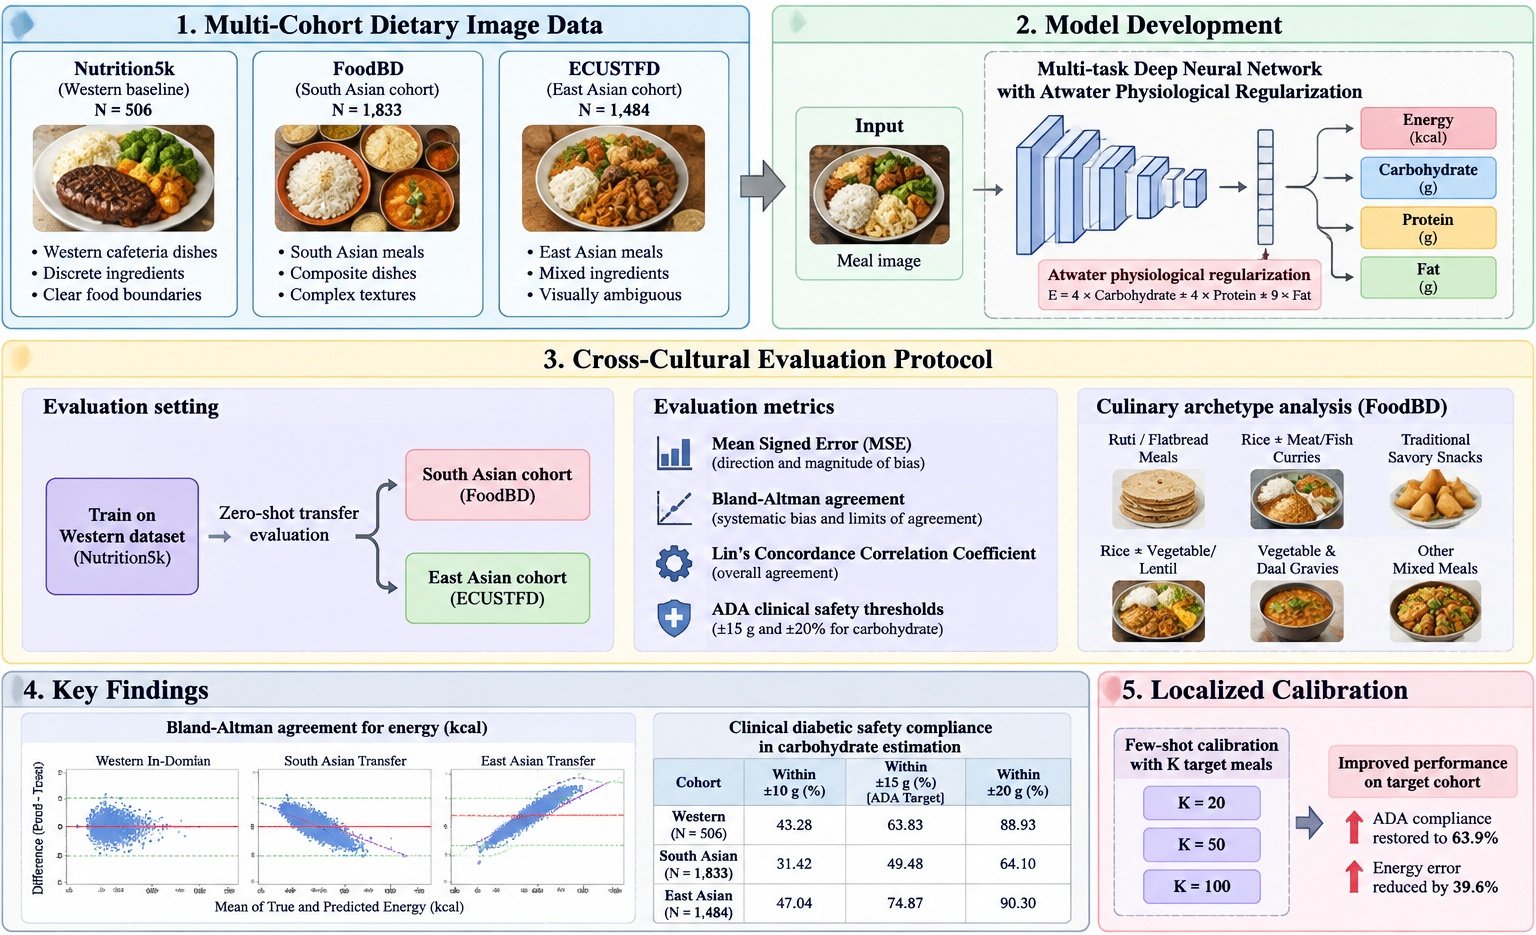
\includegraphics[width=\textwidth]{cross_cultural_framework.jpg}
\caption{\textbf{Multi-Cohort Cross-Cultural Dietary Image Analysis and Evaluation Protocol.} The end-to-end audit architecture encompasses standardized ingestion of three diverse dietary image cohorts spanning Western cafeteria dishes (Nutrition5k, $N=506$), South Asian composite meals (FoodBD, $N=1,833$), and East Asian discrete foods (ECUSTFD, $N=1,484$). A multi-task deep neural network is regularized by Atwater physiological energy conservation principles linking caloric estimation to macronutrient mass outputs. The cross-cultural evaluation protocol audits zero-shot transfer generalizability via Mean Signed Error, Bland-Altman agreement limits, Lin Concordance Correlation Coefficient, American Diabetes Association clinical carbohydrate safety compliance thresholds, and preparation archetype stratification. Mechanistic error decomposition separates surface segmentation deviations from internal nutrient density collapse, while localized few-shot recalibration demonstrates substantial error attenuation and restoration of clinical safety on target culinary cohorts.}
\label{fig:framework}
\end{figure}

\subsection{Multi-Cohort Study Population and Data Harmonization Protocol}

To evaluate cross-cultural generalizability without domain confounding, three real-world food benchmarks were assembled, spanning North American, South Asian, and East Asian culinary traditions and distinct ground-truth measurement methodologies.

The Western baseline cohort (Nutrition5k) was developed by Google Research in North American corporate cafeteria dining facilities \citep{Thames2021Nutrition5k}. Ground truth was established by precision industrial scale weighing of individual ingredients before and after dish assembly, mapped to the USDA Food and Nutrient Database for Dietary Studies (SR28). The baseline training split comprises $N=2,749$ dishes, and the official overhead test split includes $N=506$ test dishes captured by zenith RGB sensors under controlled cafeteria illumination.

The South Asian benchmark cohort (FoodBD) was curated by Ahmed et al.\ across authentic households and restaurant dining venues in Dhaka, Bangladesh \citep{Ahmed2025FoodBD}. A total of $N=1,833$ meal images containing complete nutritional annotations were evaluated. Ground-truth nutritional quantities were established by certified registered dietitians who performed visual portion estimation using standardized regional household utensils (such as katori bowls, traditional spoons, and drinking glasses) and mapped each meal component to the Food Composition Table for Bangladesh \citep{Shaheen2013BangladeshFCT}. Meals feature complex composite dishes, including heavily spiced meat and fish curries, bhunas, shak, and lentil gravies served alongside white rice or flatbread staples.

The East Asian benchmark cohort (ECUSTFD) was collected by Liang and Li at the East China University of Science and Technology \citep{Liang2017ECUSTFD}. The repository contains 2,978 high-resolution food images. To match the zenith viewing perspective of Nutrition5k and FoodBD, all $N=1,484$ top-view images were extracted. Ground-truth food mass in grams and volumetric boundaries were measured on precision digital balances with physical circular calibration tokens, and nutritional values were linked via the Chinese Food Composition Tables \citep{Yang2009ChinaFCT}. Items primarily represent discrete dishes, steamed buns, fruits, and snacks.

To ensure complete interoperability across heterogeneous annotation sources, all three cohorts were ingested into a unified data contract enforcing thirteen invariant attributes: \texttt{sample\_id}, \texttt{dataset\_name}, \texttt{cultural\_domain}, \texttt{image\_filename}, \texttt{dish\_name}, \texttt{mass\_g}, \texttt{energy\_kcal}, \texttt{protein\_g}, \texttt{fat\_g}, \texttt{carb\_g}, \texttt{provenance\_type}, \texttt{fct\_source}, and \texttt{composite\_type}.

\subsection{Problem Formulation and Multi-Task Network Architecture}

Let $\mathbf{X} \in \mathbb{R}^{3 \times H \times W}$ denote an input RGB meal photograph with spatial dimensions $H = W = 224$ pixels. The objective of dietary computer vision is to learn a mapping $f: \mathbf{X} \mapsto \hat{\mathbf{y}}$, where $\hat{\mathbf{y}}$ is a continuous vector spanning five essential nutritional quantities:
\begin{equation}
    \label{eq:output_vector}
    \hat{\mathbf{y}} = \left[ \hat{M}, \hat{E}, \hat{P}, \hat{F}, \hat{C} \right]^T \in \mathbb{R}_{\ge 0}^5
\end{equation}
In Eq.~\ref{eq:output_vector}, $\hat{M}$ denotes predicted total meal mass in grams, $\hat{E}$ represents predicted dietary energy in kilocalories, $\hat{P}$ denotes predicted protein mass in grams, $\hat{F}$ corresponds to predicted total fat mass in grams, and $\hat{C}$ signifies predicted carbohydrate mass in grams.

In complex biomedical estimation tasks, multi-task learning paradigms have demonstrated notable efficacy in capturing shared visual representations across correlated physiological outputs \citep{Wen2026MTLCS}. The network architecture couples a convolutional feature extractor with a multi-stage non-linear projection head. Feature extraction is performed via a deep residual network (ResNet-50) \citep{He2016ResNet} pre-trained on ImageNet. For an input photograph $\mathbf{X}$, spatial feature representations from the final residual block are pooled through a global average pooling layer, yielding a compact visual latent embedding $\mathbf{h} = f_\theta(\mathbf{X}) \in \mathbb{R}^{2048}$.

To map the high-dimensional visual embedding $\mathbf{h}$ into correlated nutritional targets, a dedicated regression head $g_\phi$ is constructed with two successive fully connected transformation blocks. The first intermediate projection transforms $\mathbf{h}$ into a 512-dimensional hidden state via Eq.~\ref{eq:projection_head_one}:
\begin{equation}
    \label{eq:projection_head_one}
    \mathbf{h}_1 = \text{Dropout}_{0.2}\left( \text{SiLU}\left( \text{BatchNorm}\left( \mathbf{W}_1 \mathbf{h} + \mathbf{b}_1 \right) \right) \right)
\end{equation}
where $\mathbf{W}_1 \in \mathbb{R}^{512 \times 2048}$ represents the weight matrix, $\mathbf{b}_1 \in \mathbb{R}^{512}$ is the bias vector, $\text{BatchNorm}(\cdot)$ stabilizes intermediate gradient distributions across heterogeneous nutrient scales, $\text{SiLU}(u) = u \cdot \sigma(u)$ provides continuous non-linear activation, and $\text{Dropout}_{0.2}(\cdot)$ applies a $20\%$ drop rate to prevent feature co-adaptation during training.

A second projection block compresses $\mathbf{h}_1$ into a 128-dimensional latent representation via Eq.~\ref{eq:projection_head_two}:
\begin{equation}
    \label{eq:projection_head_two}
    \mathbf{h}_2 = \text{Dropout}_{0.2}\left( \text{SiLU}\left( \text{BatchNorm}\left( \mathbf{W}_2 \mathbf{h}_1 + \mathbf{b}_2 \right) \right) \right)
\end{equation}
with weight matrix $\mathbf{W}_2 \in \mathbb{R}^{128 \times 512}$ and bias $\mathbf{b}_2 \in \mathbb{R}^{128}$. Finally, the terminal output vector is generated via a linear projection constrained by a non-negative activation in Eq.~\ref{eq:terminal_output}:
\begin{equation}
    \label{eq:terminal_output}
    \hat{\mathbf{y}} = \text{ReLU}\left( \mathbf{W}_3 \mathbf{h}_2 + \mathbf{b}_3 \right)
\end{equation}
where $\mathbf{W}_3 \in \mathbb{R}^{5 \times 128}$ and $\mathbf{b}_3 \in \mathbb{R}^5$. The terminal rectified linear unit $\text{ReLU}(u) = \max(0, u)$ guarantees that all estimated nutritional masses and energy values remain strictly non-negative, preventing physiologically impossible negative estimates.

\subsection{Physiological Regularization and Composite Training Objective}

Standard unconstrained regression networks frequently generate predictions that violate fundamental thermodynamic principles, such as predicting high caloric energy despite near-zero macronutrient masses. To eliminate unphysiological predictions, we incorporated an inductive bias based on the heat of combustion factors established by Atwater \citep{Atwater1900Physiological}. For any meal, theoretical dietary energy is bounded by the macronutrient composition:
\begin{equation}
    \label{eq:atwater_consistency}
    \hat{E}_{\text{Atwater}} = 4.0 \hat{P} + 9.0 \hat{F} + 4.0 \hat{C}
\end{equation}
In Eq.~\ref{eq:atwater_consistency}, $4.0$\,kcal/g serves as the energetic equivalent for protein and carbohydrates, while $9.0$\,kcal/g corresponds to dietary lipids.

The physiological consistency loss penalizes discrepancies between the directly predicted energy $\hat{E}$ and the Atwater equivalent $\hat{E}_{\text{Atwater}}$ across each mini-batch of size $B$ via Eq.~\ref{eq:atwater_loss}:
\begin{equation}
    \label{eq:atwater_loss}
    \mathcal{L}_{\text{Atwater}} = \frac{1}{B} \sum_{i=1}^B \ell_\delta \left( \hat{E}_i - \left( 4.0 \hat{P}_i + 9.0 \hat{F}_i + 4.0 \hat{C}_i \right) \right)
\end{equation}
In Eq.~\ref{eq:atwater_loss}, $\ell_\delta(\cdot)$ represents the Smooth $L_1$ Huber loss function defined in Eq.~\ref{eq:huber_loss}:
\begin{equation}
    \label{eq:huber_loss}
    \ell_\delta(u) = \begin{cases} 
    \frac{1}{2} u^2 & \text{if } |u| < \delta \\ 
    \delta \left( |u| - \frac{1}{2} \delta \right) & \text{otherwise} 
    \end{cases}
\end{equation}
In Eq.~\ref{eq:huber_loss}, the threshold parameter is set to $\delta = 1.0$. This formulation provides quadratic penalization for small deviations while bounding gradient magnitudes against extreme outliers.

Because target endpoints span widely differing physical scales (total mass and energy reach several hundred units, whereas fat and protein span tens of units), raw target losses would disproportionately prioritize mass over macronutrients. To balance gradient contributions across all five endpoints, ground truth and predicted vectors were standardized via z-score normalization:
\begin{equation}
    \label{eq:target_norm}
    z_{i,j} = \frac{y_{i,j} - \mu_j^{\text{train}}}{\sigma_j^{\text{train}}}, \quad \hat{z}_{i,j} = \frac{\hat{y}_{i,j} - \mu_j^{\text{train}}}{\sigma_j^{\text{train}}}
\end{equation}
In Eq.~\ref{eq:target_norm}, $j \in \{1, \dots, 5\}$ indexes the five nutritional targets, and $\mu_j^{\text{train}}$ and $\sigma_j^{\text{train}}$ represent the sample mean and standard deviation computed strictly on the training partition. Using the normalized representations from Eq.~\ref{eq:target_norm}, the primary supervised regression loss is defined in Eq.~\ref{eq:reg_loss}:
\begin{equation}
    \label{eq:reg_loss}
    \mathcal{L}_{\text{reg}} = \frac{1}{B} \sum_{i=1}^B \sum_{j=1}^5 \ell_\delta \left( \hat{z}_{i,j} - z_{i,j} \right)
\end{equation}
The composite training objective combines the standardized regression loss from Eq.~\ref{eq:reg_loss} with the Atwater physiological penalty from Eq.~\ref{eq:atwater_loss} via Eq.~\ref{eq:total_loss}:
\begin{equation}
    \label{eq:total_loss}
    \mathcal{L}_{\text{total}} = \mathcal{L}_{\text{reg}} + \lambda_{\text{Atwater}} \mathcal{L}_{\text{Atwater}}
\end{equation}
where $\lambda_{\text{Atwater}} = 0.05$ governs the strength of the physiological constraint.

The baseline model was trained exclusively on the Western Nutrition5k training cohort ($N=2,749$ dishes) for 20 epochs using the Adam optimizer with an initial learning rate of $10^{-4}$, weight decay of $10^{-4}$, and mini-batch size of 32 on an NVIDIA RTX 2080 Ti GPU (11\,GB VRAM). Checkpoint selection was determined by the lowest loss on the official Nutrition5k validation split.

\subsection{Cross-Cultural Zero-Shot Transfer and Information Isolation}

To audit cross-cultural generalizability without artificial data leakage, we enforced a strict non-pooling protocol. Datasets were never combined, shuffled, or randomly split across cultural boundaries. In clinical deployment, consumer health applications trained on centralized high-income datasets are downloaded globally without prior localized re-training. Merging datasets would obscure culture-specific failure modes and yield artificially optimistic performance estimates.

Consequently, the Western-trained model was evaluated in zero-shot transfer mode across three independent cultural cohorts. The Western in-domain audit utilized all $N=506$ official Nutrition5k overhead test dishes to establish the upper-bound performance baseline. The South Asian transfer audit evaluated all $N=1,833$ FoodBD test meals to characterize transfer performance on composite, gravied culinary preparations. The East Asian transfer audit evaluated all $N=1,484$ ECUSTFD overhead images to audit model behavior on discrete single-item foods and regional snacks.
During cross-cultural evaluation, network parameters $\theta, \phi$ and batch normalization running statistics were kept entirely frozen. No target images, labels, or target-domain statistical moments were accessible during feature extraction or prediction.

\subsection{Directional Systematic Bias and Statistical Agreement Metrics}

In clinical dietary assessment, non-directional error metrics (such as MAE and RMSE) conceal whether an algorithm consistently under-reports or over-reports nutritional intake. To expose directional distortion, we formalized directional systematic bias through Mean Signed Error (MSE):
\begin{equation}
    \label{eq:mean_signed_bias}
    \text{Bias} = \frac{1}{N} \sum_{i=1}^N \left( \hat{y}_i - y_i \right)
\end{equation}
In Eq.~\ref{eq:mean_signed_bias}, $y_i$ represents the true nutritional quantity and $\hat{y}_i$ is the predicted value for meal $i$. A positive bias indicates systematic overestimation, whereas a negative bias denotes systematic underestimation.

To evaluate relative directional distortion scaled to meal size, Mean Percentage Error (MPE) was calculated:
\begin{equation}
    \label{eq:mpe}
    \text{MPE} = \frac{1}{N} \sum_{i=1}^N \left( \frac{\hat{y}_i - y_i}{y_i} \right) \times 100\%
\end{equation}
A two-tailed paired Student's $t$-test was conducted on the meal-level difference series $d_i = \hat{y}_i - y_i$ to evaluate the null hypothesis of zero systematic bias ($H_0: \mu_d = 0$).

Medical measurement agreement was analyzed using the Bland-Altman method \citep{Bland1986BlandAltman}. Let $\bar{d} = \frac{1}{N}\sum_{i=1}^N d_i$ denote the mean difference, and let $s_d = \sqrt{\frac{1}{N-1}\sum_{i=1}^N (d_i - \bar{d})^2}$ be the sample standard deviation. The $95\%$ Limits of Agreement (LoA) are defined in Eq.~\ref{eq:loa}:
\begin{equation}
    \label{eq:loa}
    \text{LoA} = \left[ \bar{d} - 1.96 s_d, \quad \bar{d} + 1.96 s_d \right]
\end{equation}
To determine whether bias varied systematically with meal size, proportional bias was audited via ordinary least squares regression of measurement differences against pair averages in Eq.~\ref{eq:ols_proportional_bias}:
\begin{equation}
    \label{eq:ols_proportional_bias}
    d_i = \beta_0 + \beta_1 \left( \frac{\hat{y}_i + y_i}{2} \right) + \epsilon_i
\end{equation}
A statistically significant slope ($\beta_1 \ne 0$, $p < 0.05$) demonstrates proportional bias, indicating that estimation discrepancies scale with portion size.

Concordance between predictions and reference values was assessed via Lin's Concordance Correlation Coefficient (CCC) \citep{Lin1989CCC}:
\begin{equation}
    \label{eq:lin_ccc}
    \rho_c = \frac{2 \sigma_{y\hat{y}}}{\sigma_y^2 + \sigma_{\hat{y}}^2 + \left( \mu_y - \mu_{\hat{y}} \right)^2}
\end{equation}
In Eq.~\ref{eq:lin_ccc}, $\mu_y$ and $\mu_{\hat{y}}$ are the means, $\sigma_y^2$ and $\sigma_{\hat{y}}^2$ are the variances, and $\sigma_{y\hat{y}}$ is the sample covariance. Lin CCC measures both precision (correlation) and accuracy (distance from the $45^\circ$ line of identity), providing a unified index ranging from $-1.0$ to $+1.0$.

\subsection{Clinical Safety Criteria for Diabetic Carbohydrate Counting}

For individuals managing diabetes with prandial insulin therapy, accurate carbohydrate counting is essential for insulin dose titration. Clinical guidelines from the American Diabetes Association (ADA) and clinical bolus algorithms utilize an insulin-to-carbohydrate ratio (typically 1 unit of rapid-acting insulin per 10 to 15 grams of carbohydrate) \citep{ADA2025CarbCounting,Bell2015CarbInsulin}. Estimation discrepancies exceeding $\pm 15$\,g carbohydrate translate directly into insulin dosing errors of $1.0$ to $1.5$ units, creating serious risks of postprandial hypoglycemia or sustained hyperglycemia.

To translate computer vision accuracy into clinical safety endpoints, we defined the absolute carbohydrate safety compliance rate in Eq.~\ref{eq:clinical_compliance_abs}:
\begin{equation}
    \label{eq:clinical_compliance_abs}
    \text{Comp}_{\le \theta} = \frac{1}{N} \sum_{i=1}^N \mathbb{I}\left( |\hat{C}_i - C_i| \le \theta \right) \times 100\%
\end{equation}
where $\mathbb{I}(\cdot)$ is the indicator function, and $\theta \in \{10, 15, 20\}$\,g represents the clinical tolerance threshold. The primary safety endpoint was specified as $\theta = 15$\,g, with $\theta = 10$\,g representing strict high-sensitivity insulin control and $\theta = 20$\,g representing a permissive margin.

To account for varying meal sizes, relative percentage compliance was evaluated via Eq.~\ref{eq:clinical_compliance_rel}:
\begin{equation}
    \label{eq:clinical_compliance_rel}
    \text{Comp}_{\le \eta\%} = \frac{1}{N} \sum_{i=1}^N \mathbb{I}\left( \frac{|\hat{C}_i - C_i|}{C_i} \le \eta \right) \times 100\%
\end{equation}
where $\eta \in \{0.15, 0.20\}$ denotes relative error bounds of $\pm 15\%$ and $\pm 20\%$.

\subsection{Mechanistic Error Decomposition Formulation}

Cross-cultural estimation errors may arise either from inaccurate portion volume estimation (geometric segmentation error) or from inaccurate nutrient density estimation per unit food mass (biochemical composition blindness). To isolate these mechanisms, we formulated an orthogonal error decomposition for dietary carbohydrate.

True carbohydrate mass $C$ is the product of total meal mass $M$ and carbohydrate density $D = C / M$, as expressed in Eq.~\ref{eq:carb_product}:
\begin{equation}
    \label{eq:carb_product}
    C = M \cdot D
\end{equation}
Similarly, predicted carbohydrate mass $\hat{C}$ equals predicted mass $\hat{M}$ multiplied by predicted density $\hat{D} = \hat{C} / \hat{M}$. Subtracting reference intake in Eq.~\ref{eq:carb_product} from predicted intake yields the error decomposition in Eq.~\ref{eq:error_decomposition}:
\begin{equation}
    \label{eq:error_decomposition}
    \hat{C} - C = \underbrace{(\hat{M} - M) D}_{\Delta_{\text{mass}}} + \underbrace{M (\hat{D} - D)}_{\Delta_{\text{density}}} + \underbrace{(\hat{M} - M)(\hat{D} - D)}_{\Delta_{\text{interaction}}}
\end{equation}
In Eq.~\ref{eq:error_decomposition}, $\Delta_{\text{mass}}$ isolates the error attributable to meal mass deviation holding true density constant, $\Delta_{\text{density}}$ quantifies the error resulting from internal nutrient density misattribution holding true mass constant, and $\Delta_{\text{interaction}}$ captures the second-order coupling term between mass and density errors. This mathematical attribution isolates whether cross-cultural failures stem from surface segmentation boundaries or internal chemical composition blindness.

\subsection{Few-Shot Localized Calibration Protocol}

To evaluate whether cross-cultural systematic bias can be remediated without retraining the deep visual backbone, we formulated an affine recalibration protocol. Collecting large-scale nutrition datasets with laboratory scale weighing is resource-intensive, whereas collecting a modest local calibration set of $K \in \{20, 50, 100\}$ meals is feasible for regional healthcare providers.

For each nutritional endpoint $y \in \{M, E, P, F, C\}$, an affine calibration mapping is learned on the calibration bank while keeping visual parameters $\theta, \phi$ frozen:
\begin{equation}
    \label{eq:few_shot_calibration}
    \hat{y}_{\text{cal}} = \alpha \hat{y} + \beta
\end{equation}
In Eq.~\ref{eq:few_shot_calibration}, scaling parameter $\alpha \in \mathbb{R}$ and intercept $\beta \in \mathbb{R}$ are estimated via ordinary least squares regression on the $K$ calibration pairs $(y_k, \hat{y}_k)_{k=1}^K$. The calibrated predictions are then evaluated on an independent, held-out target test partition ($N=180$) to measure bias attenuation and recovery of clinical safety compliance.

\section{Results}

\subsection{Cross-Cultural Performance Degradation and Directional Bias}

Cross-cultural transfer of the multi-task vision model from Western cafeteria dishes to South Asian and East Asian diets induced marked performance degradation across all five nutritional endpoints, accompanied by pronounced directional systematic bias (Table~\ref{tab:evaluation_matrix}).

In-domain evaluation on Western dishes (Nutrition5k, $N=506$) established the upper-bound performance of the model. On this cohort, the network achieved balanced carbohydrate estimation with a Mean Signed Bias of $+0.94$\,g, which was not statistically significantly different from zero ($p = 0.176$, evaluated via Eq.~\ref{eq:mean_signed_bias}). Concordance was robust for total dietary energy, yielding a Lin CCC of $0.694$ with an MAE of $120.81$\,kcal, and for total meal mass, yielding a Lin CCC of $0.660$ with an MAE of $92.10$\,g (Eq.~\ref{eq:lin_ccc}). Total fat estimation demonstrated minimal signed bias ($-0.09$\,g, $p = 0.881$), while protein estimation exhibited an MAE of $13.74$\,g with a minor positive bias ($+2.36$\,g, $p = 1.39 \times 10^{-3}$).

Upon zero-shot transfer to South Asian meals (FoodBD, $N=1,833$), the model exhibited a severe, statistically catastrophic negative bias in carbohydrate estimation. As detailed in Table~\ref{tab:evaluation_matrix}, the Mean Signed Bias reached $-18.18$\,g, corresponding to a Mean Percentage Error of $-22.01\%$ ($p = 8.64 \times 10^{-206}$, evaluated via Eq.~\ref{eq:mpe}). Authentic South Asian meals in this cohort contained an average of $38.8 \pm 22.4$\,g of carbohydrate derived from boiled rice, flatbreads, and legume curries. In contrast, the Western-trained network predicted an invariant, constricted mean of only $20.6 \pm 2.8$\,g, regressing toward its Western cafeteria training prior ($19.7 \pm 17.5$\,g) and failing to perceive dense starches dispersed within gravies. Consequently, the carbohydrate MAE escalated from $12.51$\,g in-domain to $20.43$\,g under transfer, representing a $63.3\%$ error increase, while Lin CCC collapsed from $0.225$ to $0.018$. Total meal mass error simultaneously expanded, with mass MAE increasing from $92.10$\,g to $164.56$\,g (a $78.7\%$ degradation) and exhibiting a substantial positive bias of $+141.39$\,g ($p = 1.56 \times 10^{-302}$). Total energy MAE increased by $26.4\%$ to $152.65$\,kcal, accompanied by an overestimation bias of $+100.36$\,kcal ($p = 9.51 \times 10^{-128}$).

On East Asian images (ECUSTFD, $N=1,484$), the model displayed a different manifestation of cultural bias characterized by large positive energy and macronutrient overestimation. Because ECUSTFD comprises single-portion fruits, steamed buns, and discrete snacks with a true mean energy of only $120.6 \pm 76.4$\,kcal, the model over-projected caloric content toward the multi-component Western cafeteria baseline ($255.8 \pm 212.4$\,kcal). This prior dominance produced a positive energy bias of $+134.73$\,kcal ($p < 10^{-300}$, MPE $+241.38\%$), causing the energy Lin CCC to collapse to $0.004$. Protein and fat were likewise severely overestimated, with protein exhibiting an MAE of $16.12$\,g ($+16.12$\,g bias, $p < 10^{-300}$, MPE $+1376.07\%$) and fat exhibiting an MAE of $10.21$\,g ($+9.73$\,g bias, $p < 10^{-300}$, MPE $+2743.04\%$). East Asian carbohydrate estimation exhibited moderate negative bias ($-4.11$\,g, $p = 9.10 \times 10^{-30}$), with an MAE of $11.28$\,g and a Lin CCC of $0.007$.

In summary, cross-cultural deployment revealed that global error metrics mask profound directional shifts: Western models under-predict dense mixed carbohydrates in South Asian diets while over-projecting caloric volume onto small East Asian portions. Because aggregate correlation metrics cannot characterize whether estimation errors expand proportionally across meal sizes, individual clinical concordance requires detailed Bland-Altman agreement analysis.

\begin{table}[tbp]
\centering
\small
\caption{\textbf{Cross-Cultural Evaluation Matrix for Dietary Energy and Macronutrient Estimation.} Empirical performance of the ResNet-50 multi-task model trained on Western cafeteria dishes (Nutrition5k) and evaluated in-domain and zero-shot across South Asian (FoodBD) and East Asian (ECUSTFD) cohorts ($N=3,823$ total images). Best values per metric within each nutrient target are highlighted in bold.}
\label{tab:evaluation_matrix}
\vspace{4pt}
\resizebox{\textwidth}{!}{
\begin{tabular}{llrrrrrrr}
\toprule
\textbf{Target Cohort} & \textbf{Nutrient} & \textbf{MAE} & \textbf{RMSE} & \textbf{MAPE (\%)} & \textbf{Mean Bias} & \textbf{MPE (\%)} & \textbf{Bias $p$-value} & \textbf{Lin CCC} \\
\midrule
\multirow{5}{*}{\parbox{2.8cm}{\textbf{Western}\\(Nutrition5k, $N=506$)}} 
 & Mass (g)          & \textbf{92.10}  & \textbf{110.11} & 215.40 & \textbf{+68.36}  & +209.74 & $2.29 \times 10^{-55}$  & \textbf{0.660} \\
 & Energy (kcal)     & \textbf{120.81} & \textbf{144.59} & 380.53 & \textbf{+75.80}  & +371.54 & $3.94 \times 10^{-37}$  & \textbf{0.694} \\
 & Protein (g)       & 13.74  & 16.66  & 865.24 & \textbf{+2.36}   & +840.12 & $1.39 \times 10^{-3}$   & \textbf{0.274} \\
 & Fat (g)           & 10.63  & 14.03  & 1482.66& \textbf{-0.09}   & +1449.12& \textbf{0.881 (n.s.)}   & \textbf{0.016} \\
 & Carb (g)          & 12.51  & 15.62  & 556.44 & \textbf{+0.94}   & +529.79 & \textbf{0.176 (n.s.)}   & \textbf{0.225} \\
\midrule
\multirow{5}{*}{\parbox{2.8cm}{\textbf{South Asian}\\(FoodBD, $N=1,833$)}} 
 & Mass (g)$^\dagger$& 164.56 & 194.24 & \textbf{105.37} & +141.39 & \textbf{+99.75}  & $1.56 \times 10^{-302}$ & 0.072 \\
 & Energy (kcal)     & 152.65 & 192.89 & \textbf{63.90}  & +100.36 & \textbf{+53.36}  & $9.51 \times 10^{-128}$ & 0.226 \\
 & Protein (g)       & \textbf{12.19}  & \textbf{13.64}  & \textbf{157.78} & +11.69  & \textbf{+156.06} & $< 10^{-300}$           & 0.076 \\
 & Fat (g)           & \textbf{5.05}   & \textbf{6.44}   & \textbf{200.97} & +2.74   & \textbf{+189.22} & $3.99 \times 10^{-81}$  & -0.00001 \\
 & Carb (g)          & 20.43  & 28.73  & \textbf{53.76}  & -18.18 & \textbf{-22.01} & $8.64 \times 10^{-206}$ & 0.018 \\
\midrule
\multirow{5}{*}{\parbox{2.8cm}{\textbf{East Asian}\\(ECUSTFD, $N=1,484$)}} 
 & Mass (g)          & 100.94 & 118.31 & 160.21 & +78.10  & +152.86 & $1.45 \times 10^{-186}$ & 0.015 \\
 & Energy (kcal)     & 140.91 & 154.61 & 243.10 & +134.73 & +241.38 & $< 10^{-300}$           & 0.004 \\
 & Protein (g)       & 16.12  & 16.20  & 1376.07& +16.12  & +1376.07& $< 10^{-300}$           & 0.000 \\
 & Fat (g)           & 10.21  & 10.90  & 2745.84& +9.73   & +2743.04& $< 10^{-300}$           & 0.000 \\
 & Carb (g)          & \textbf{11.28}  & \textbf{14.28}  & 152.20 & -4.11   & +110.32 & $9.10 \times 10^{-30}$  & 0.007 \\
\bottomrule
\end{tabular}
}
\vspace{2pt}
\flushleft
\scriptsize{$^\dagger$South Asian mass represents dietitian-estimated portion mass. n.s.: not statistically significant ($p > 0.05$). MPE: Mean Percentage Error. Lin CCC: Lin Concordance Correlation Coefficient.}
\end{table}

\subsection{Bland-Altman Medical Agreement Analysis}

Bland-Altman agreement analysis for total dietary energy revealed substantial cross-cultural divergence in residual dispersion and limits of agreement (Figure~\ref{fig:bland_altman_energy}). In-domain Western dishes exhibited a mean bias of $+75.8$\,kcal with $95\%$ limits of agreement spanning $[-165.8, +317.4]$\,kcal (total agreement span of $483.2$\,kcal, evaluated via Eq.~\ref{eq:loa}). Residual errors were distributed symmetrically around the mean bias line across the lower and middle caloric spectrum.

When transferred to South Asian meals (Figure~\ref{fig:bland_altman_energy}B), the agreement envelope broadened substantially to $[-222.6, +423.3]$\,kcal, spanning a total range of $645.9$\,kcal. This represents an absolute widening of $162.7$\,kcal and a $33.7\%$ increase in the uncertainty interval relative to in-domain dishes. Furthermore, ordinary least squares regression confirmed highly significant proportional bias ($p < 10^{-8}$, evaluated via Eq.~\ref{eq:ols_proportional_bias}), as evidenced by the positive regression slope line. The positive slope demonstrates that the degree of energy overestimation scaled progressively with meal portion size, generating discrepancies exceeding $+300$\,kcal on large composite platters.

On East Asian images (Figure~\ref{fig:bland_altman_energy}C), the agreement limits shifted almost entirely above the zero line to $[-16.5, +285.9]$\,kcal with a mean bias of $+134.7$\,kcal. Because true caloric content was low for most single-item foods, the network consistently over-predicted energy by more than $100$\,kcal across the entire dataset.

The resulting scatter confirms that standard correlation metrics conceal severe meal-level estimation divergence that directly impairs dietary tracking. Because meal-level divergence carries immediate implications for dietary therapy, establishing whether these estimation errors compromise clinical safety standards for diabetic carbohydrate counting is essential.

\begin{figure}[tbp]
\centering
\begin{minipage}{0.32\textwidth}
    \centering
    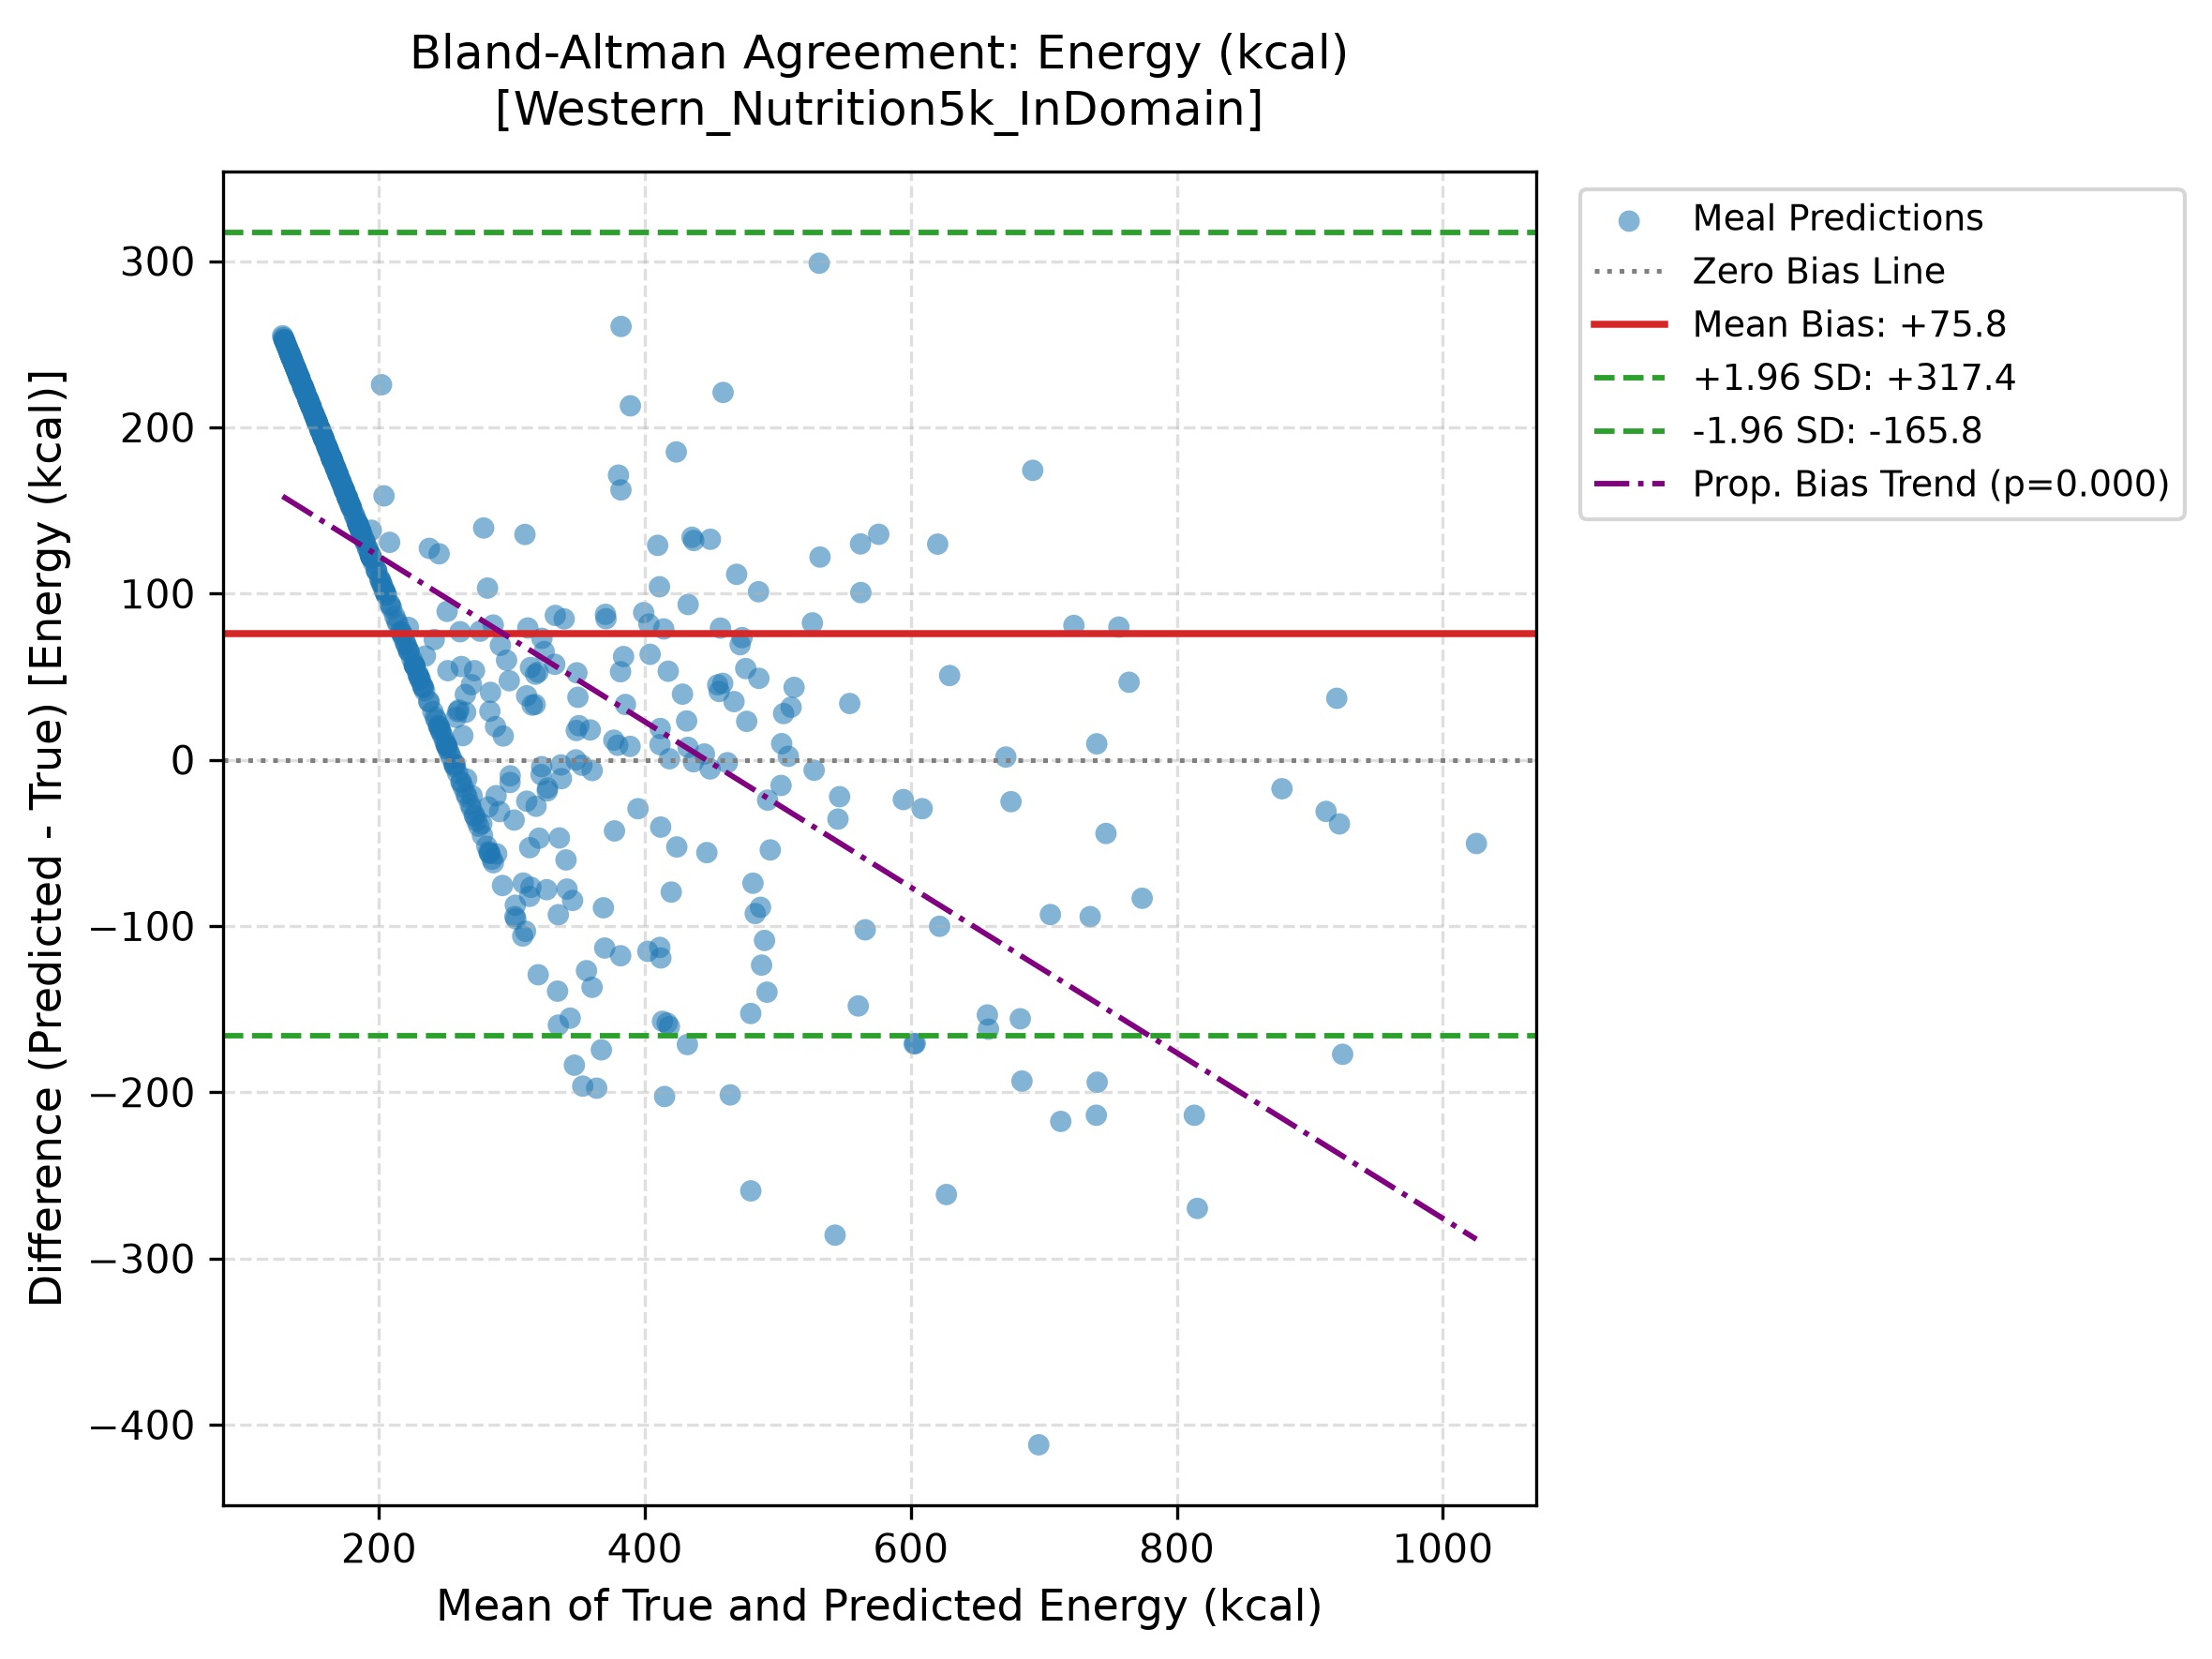
\includegraphics[width=\textwidth]{bland_altman_Western_Nutrition5k_InDomain_energy.jpg}\\
    \small \textbf{(A)} Western In-Domain
\end{minipage}
\hfill
\begin{minipage}{0.32\textwidth}
    \centering
    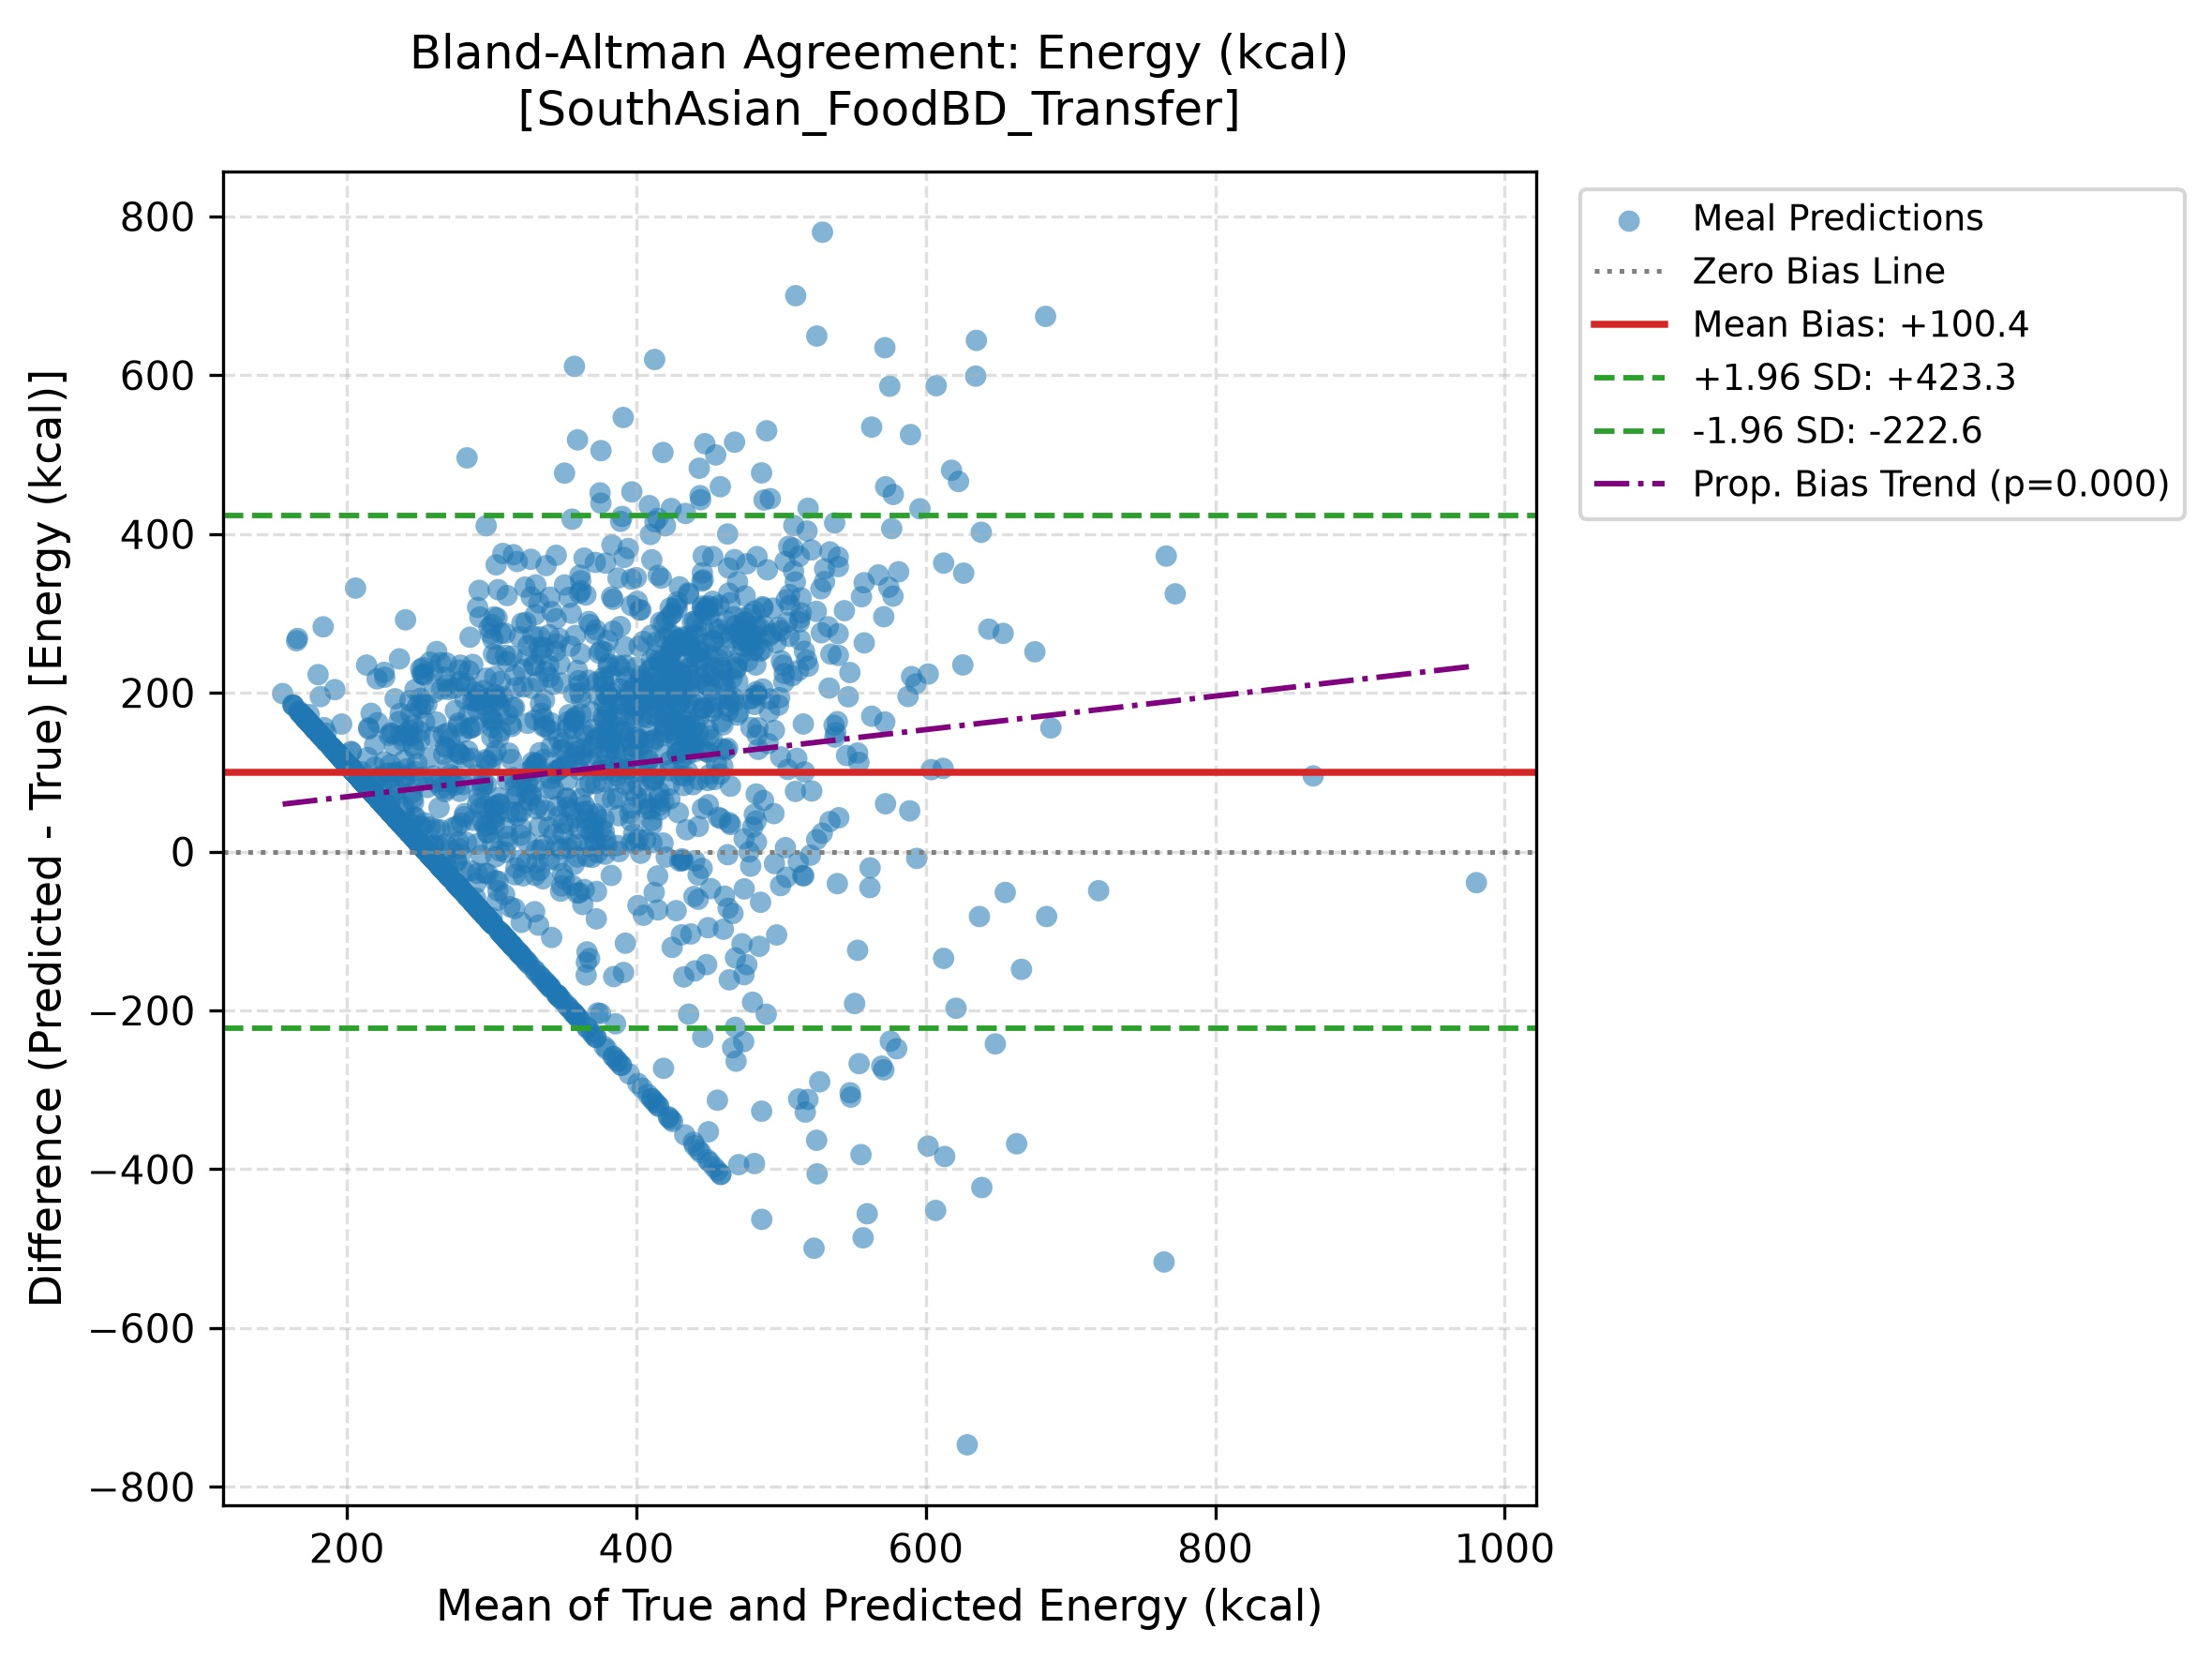
\includegraphics[width=\textwidth]{bland_altman_SouthAsian_FoodBD_Transfer_energy.jpg}\\
    \small \textbf{(B)} South Asian Transfer
\end{minipage}
\hfill
\begin{minipage}{0.32\textwidth}
    \centering
    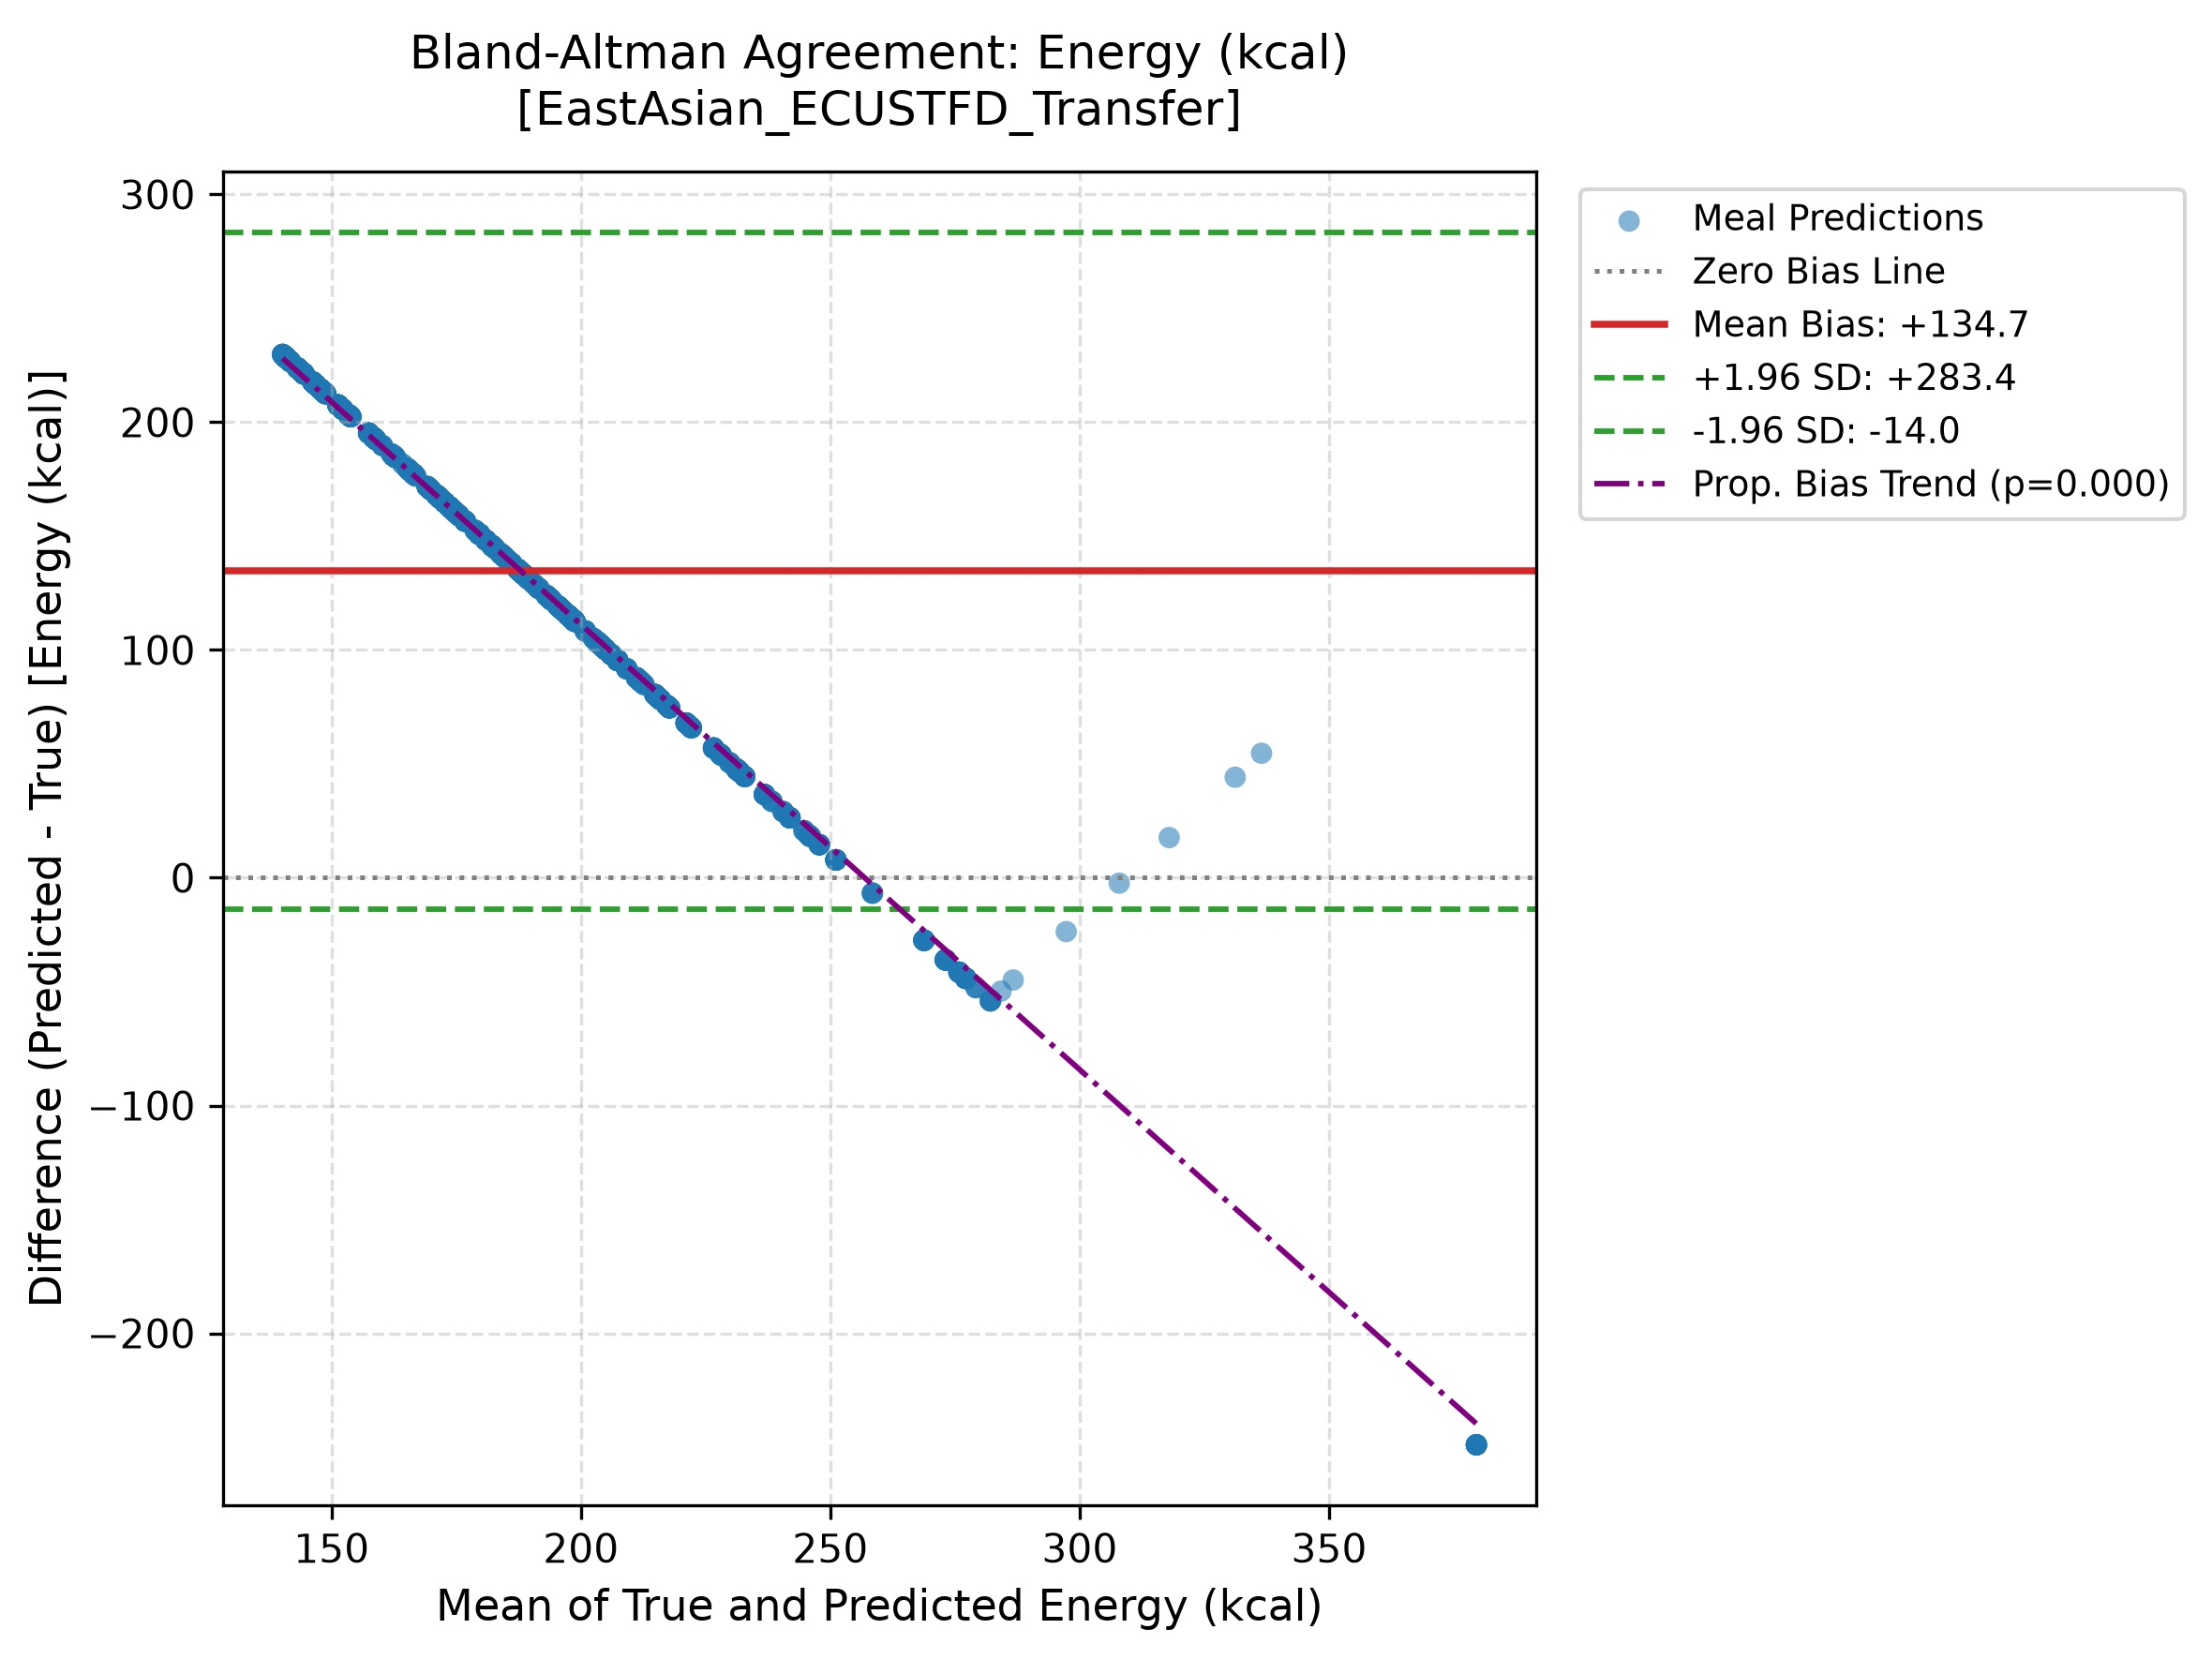
\includegraphics[width=\textwidth]{bland_altman_EastAsian_ECUSTFD_Transfer_energy.jpg}\\
    \small \textbf{(C)} East Asian Transfer
\end{minipage}
\caption{\textbf{Bland-Altman Agreement for Dietary Energy (kcal).} Comparison of predicted versus true caloric energy across the three dietary benchmarks ($N=3,823$). Red solid lines denote mean bias, whereas green dashed lines indicate $95\%$ Limits of Agreement ($\bar{d} \pm 1.96 s_d$). Purple dash-dotted lines represent linear regression trends for proportional bias.}
\label{fig:bland_altman_energy}
\end{figure}

\subsection{Clinical Compliance in Diabetic Carbohydrate Counting}

Clinical compliance with diabetic carbohydrate counting tolerances demonstrated severe cross-cultural disparities (Table~\ref{tab:clinical_safety} and Figure~\ref{fig:bland_altman_carb}). Under in-domain Western evaluation, $63.83\%$ of meal carbohydrate predictions satisfied the primary ADA clinical tolerance window ($\pm 15$\,g of true carbohydrate, evaluated via Eq.~\ref{eq:clinical_compliance_abs}), and $88.93\%$ complied with the permissive $\pm 20$\,g margin. Under the strict high-sensitivity threshold ($\pm 10$\,g, relevant for patients with high insulin sensitivity), compliance reached $43.28\%$.

In sharp contrast, transferring the model to South Asian meals resulted in a pronounced collapse in ADA clinical safety compliance, which fell to 49.48\%. This represents an absolute decrease of $14.35$ percentage points ($p < 10^{-8}$) and a relative decline of $22.5\%$. Consequently, more than half ($50.52\%$) of all South Asian meals fell outside the clinically acceptable margin for prandial insulin bolusing. Under the permissive $\pm 20$\,g threshold, South Asian compliance was restricted to $64.10\%$, trailing the Western in-domain benchmark by $24.83$ percentage points. Under the strict $\pm 10$\,g margin, compliance dropped to $31.42\%$, indicating that over two-thirds of meals would produce clinically hazardous bolus calculations in insulin-sensitive patients.

On East Asian images, compliance with the $\pm 15$\,g ADA target stood at $74.87\%$, and $90.30\%$ satisfied $\pm 20$\,g. This relatively high absolute compliance was driven by the low true carbohydrate baseline of ECUSTFD snacks ($11.28 \pm 14.28$\,g), which allowed predictions clustered around the $20$\,g prior to remain within the $\pm 15$\,g window. Conversely, relative percentage tolerances ($\pm 15\%$ and $\pm 20\%$ relative error, evaluated via Eq.~\ref{eq:clinical_compliance_rel}) were violated in over $79\%$ of cases across all three cohorts. Specifically, compliance within $\pm 20\%$ relative error was only $18.92\%$ in Western dishes, $17.86\%$ in South Asian meals, and $20.69\%$ in East Asian foods. This finding demonstrates that relative percentage metrics disproportionately penalize low-carbohydrate dishes and fail to provide stable clinical guidance without absolute margin boundaries.

The Bland-Altman agreement plots for dietary carbohydrate (Figure~\ref{fig:bland_altman_carb}) expose the directional nature of this failure. While Western dishes (Figure~\ref{fig:bland_altman_carb}A) clustered around zero bias ($+0.94$\,g), South Asian meals (Figure~\ref{fig:bland_altman_carb}B) showed a pronounced downward fan-out. As true meal carbohydrate content increased from $30$\,g to over $80$\,g, estimation discrepancies expanded to $-40$\,g and $-60$\,g, proving that the risk of insulin under-dosing is concentrated in meals with the highest glycemic load.

Because South Asian dietary practices encompass highly heterogeneous preparation methods, determining whether this downward fan-out reflects uniform model failure or distinct dish composition requires a granular audit across culinary archetypes.

\begin{table}[tbp]
\centering
\small
\caption{\textbf{Clinical Diabetic Safety Compliance in Carbohydrate Estimation.} Percentage of meals meeting strict absolute and relative clinical error tolerances for mealtime insulin calculation across Western in-domain and cross-cultural transfer cohorts ($N=3,823$ total images). Best values per column are highlighted in bold.}
\label{tab:clinical_safety}
\vspace{4pt}
\resizebox{\textwidth}{!}{
\begin{tabular}{lrrrrr}
\toprule
\textbf{Target Cohort} & \textbf{Within $\pm 10$\,g (\%)} & \textbf{Within $\pm 15$\,g (\%)} & \textbf{Within $\pm 20$\,g (\%)} & \textbf{Within $\pm 15$\% (\%)} & \textbf{Within $\pm 20$\% (\%)} \\
 & & \textbf{[ADA Target]} & & & \textbf{[Clinical Safe]} \\
\midrule
\textbf{Western} (Nutrition5k, $N=506$)   & 43.28 & 63.83 & 88.93 & 14.34 & 18.92 \\
\textbf{South Asian} (FoodBD, $N=1,833$) & 31.42 & 49.48 & 64.10 & 12.78 & 17.86 \\
\textbf{East Asian} (ECUSTFD, $N=1,484$) & \textbf{47.04} & \textbf{74.87} & \textbf{90.30} & \textbf{16.44} & \textbf{20.69} \\
\bottomrule
\end{tabular}
}
\end{table}

\begin{figure}[tbp]
\centering
\begin{minipage}{0.32\textwidth}
    \centering
    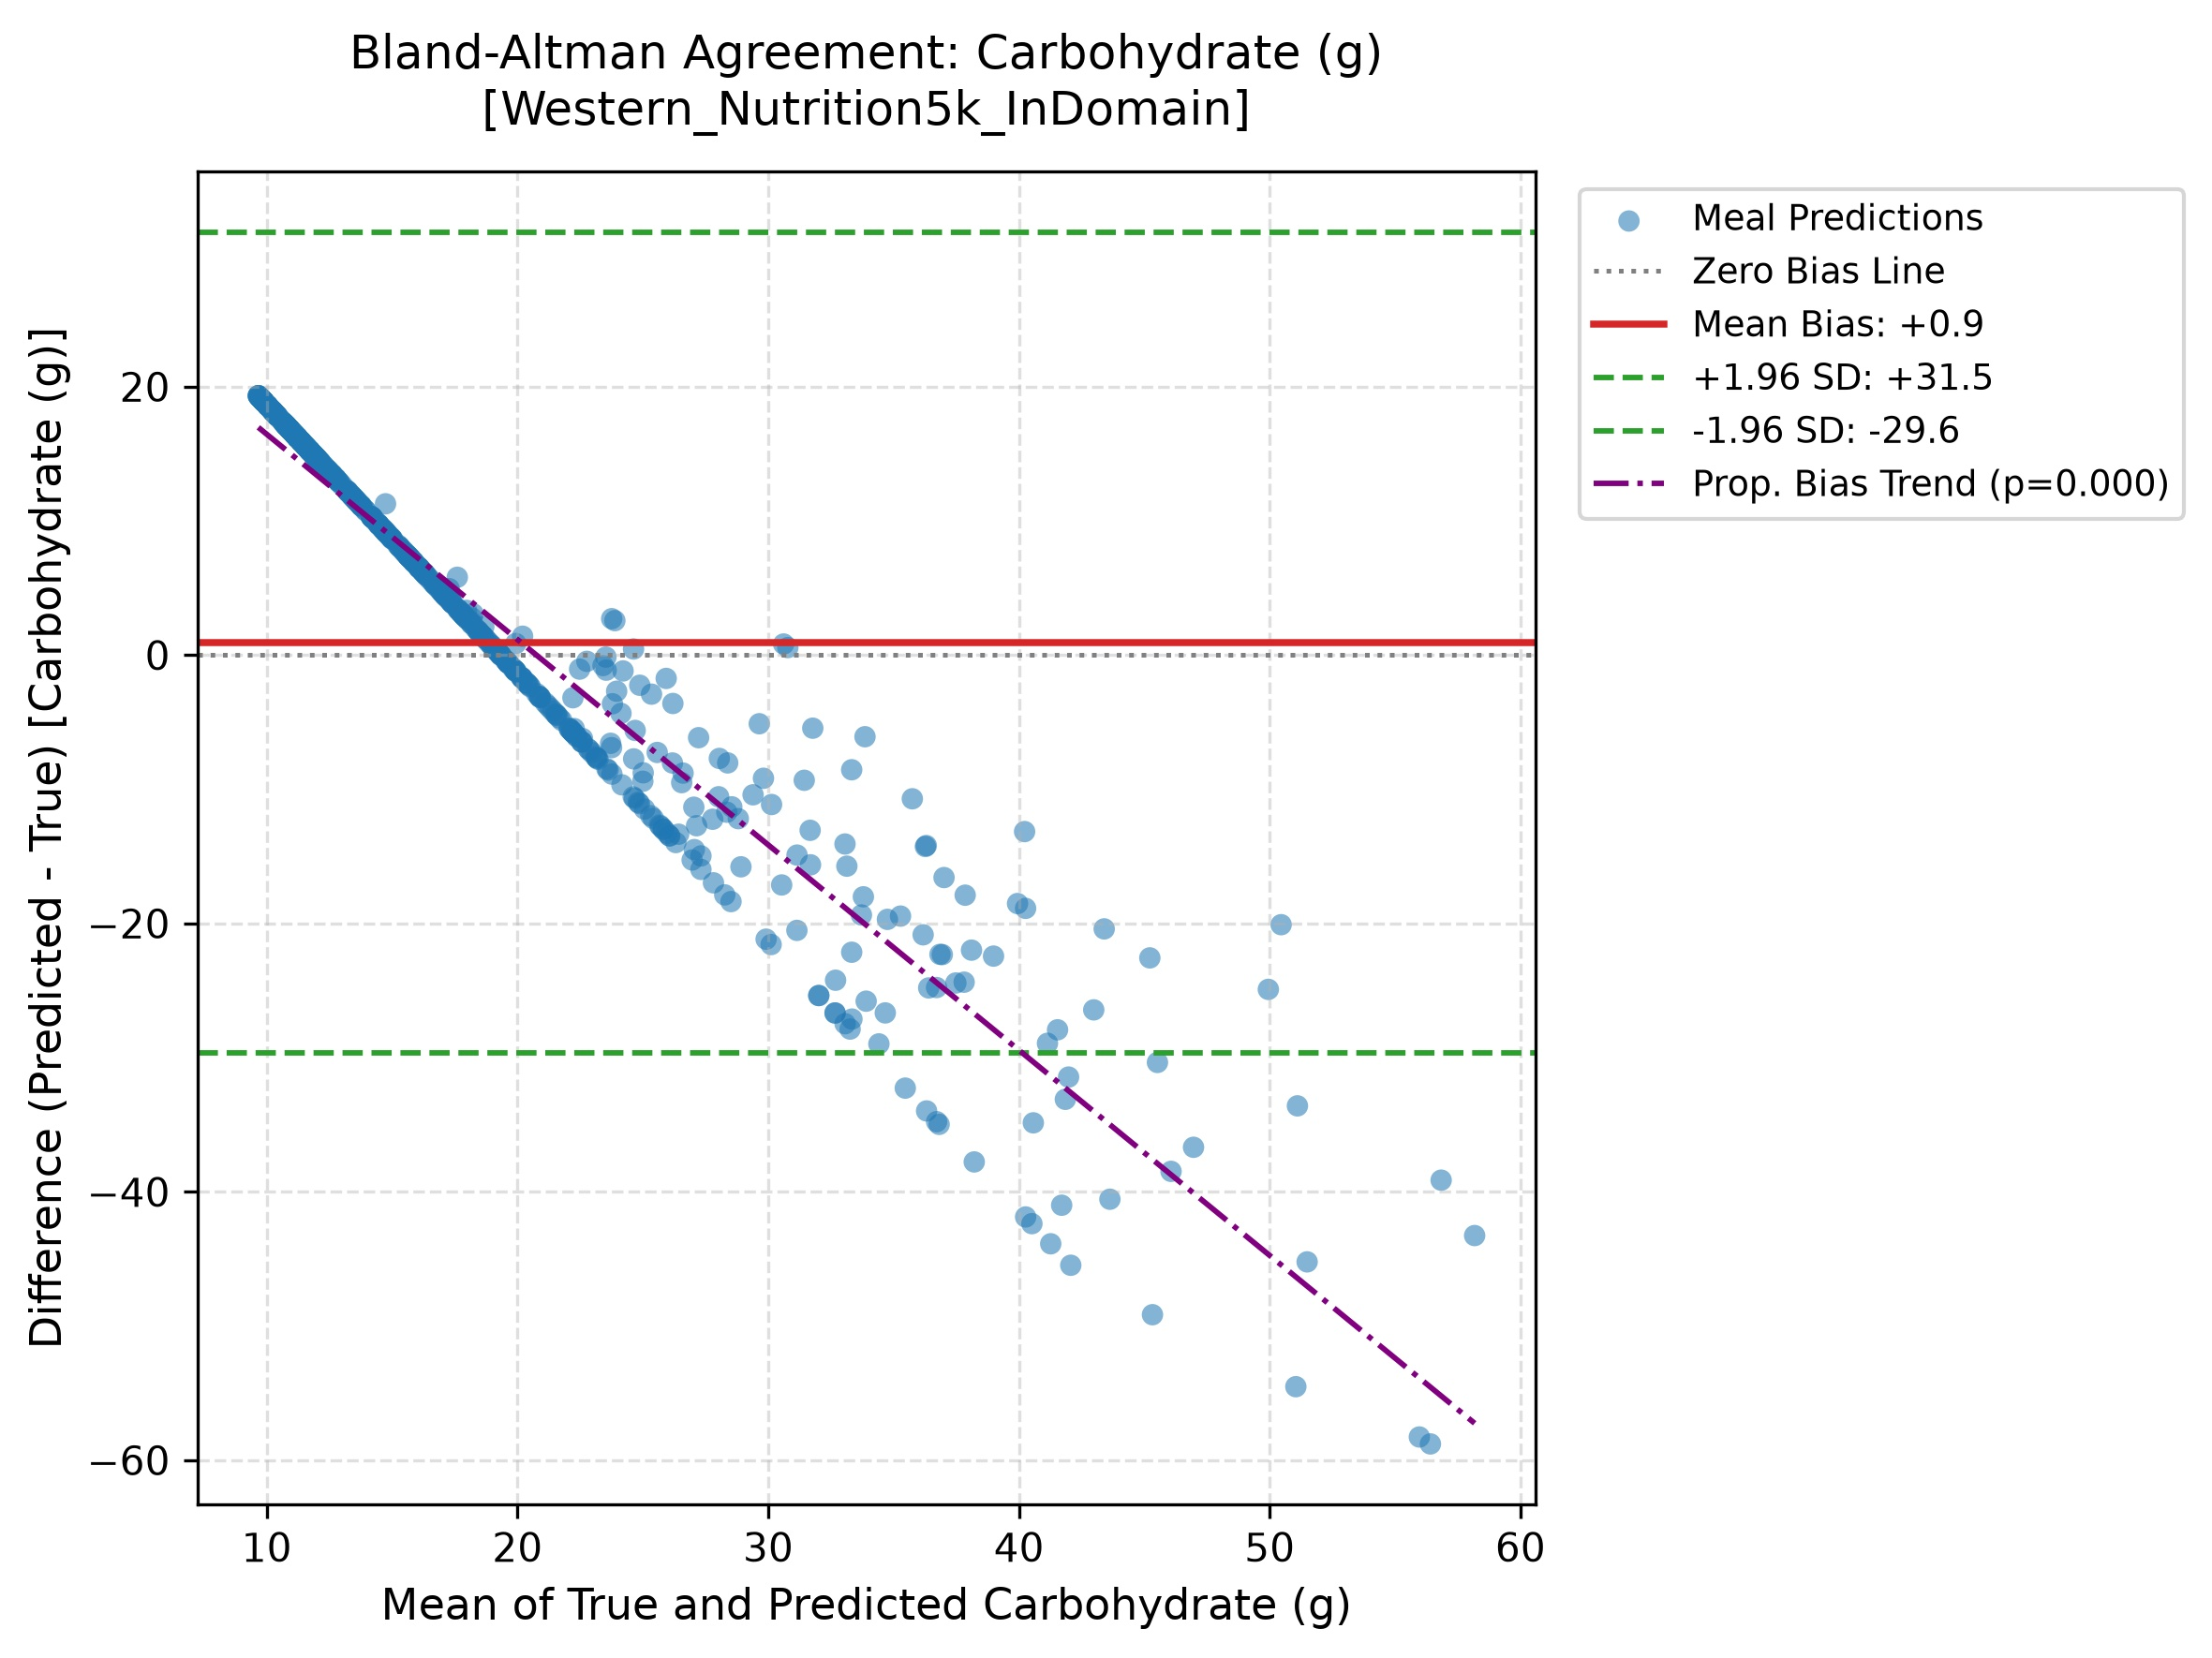
\includegraphics[width=\textwidth]{bland_altman_Western_Nutrition5k_InDomain_carb.jpg}\\
    \small \textbf{(A)} Western In-Domain
\end{minipage}
\hfill
\begin{minipage}{0.32\textwidth}
    \centering
    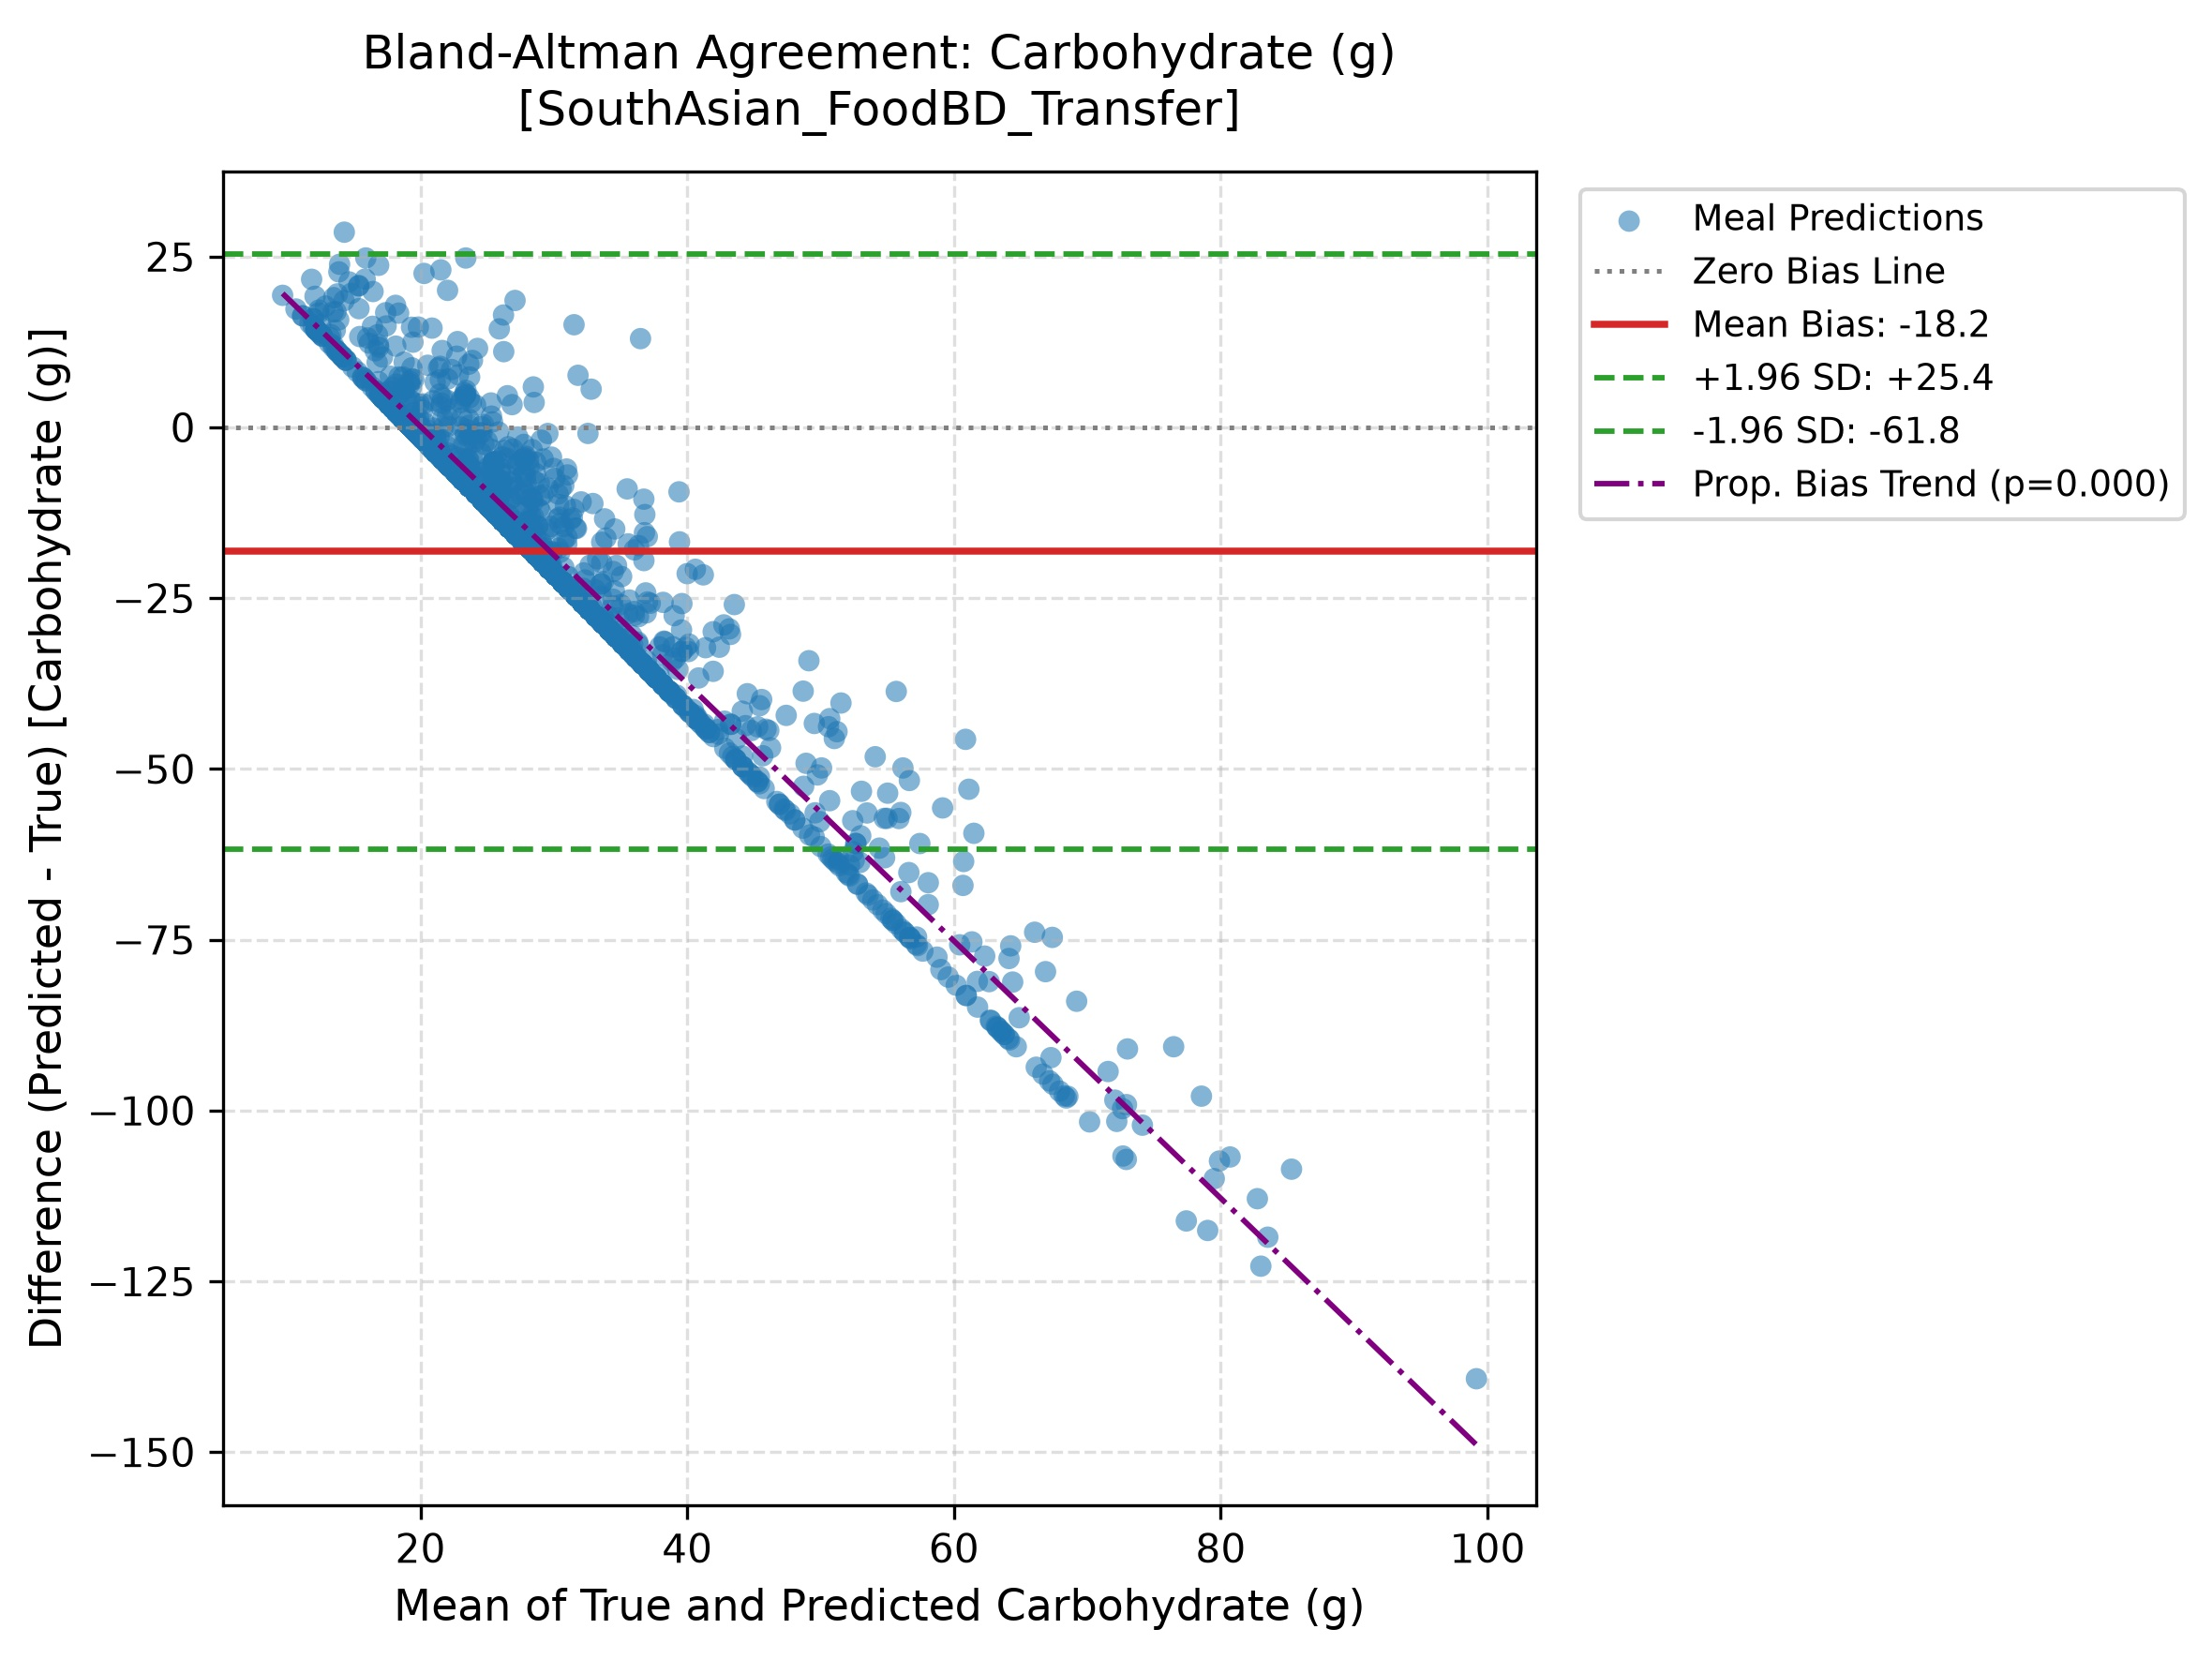
\includegraphics[width=\textwidth]{bland_altman_SouthAsian_FoodBD_Transfer_carb.jpg}\\
    \small \textbf{(B)} South Asian Transfer
\end{minipage}
\hfill
\begin{minipage}{0.32\textwidth}
    \centering
    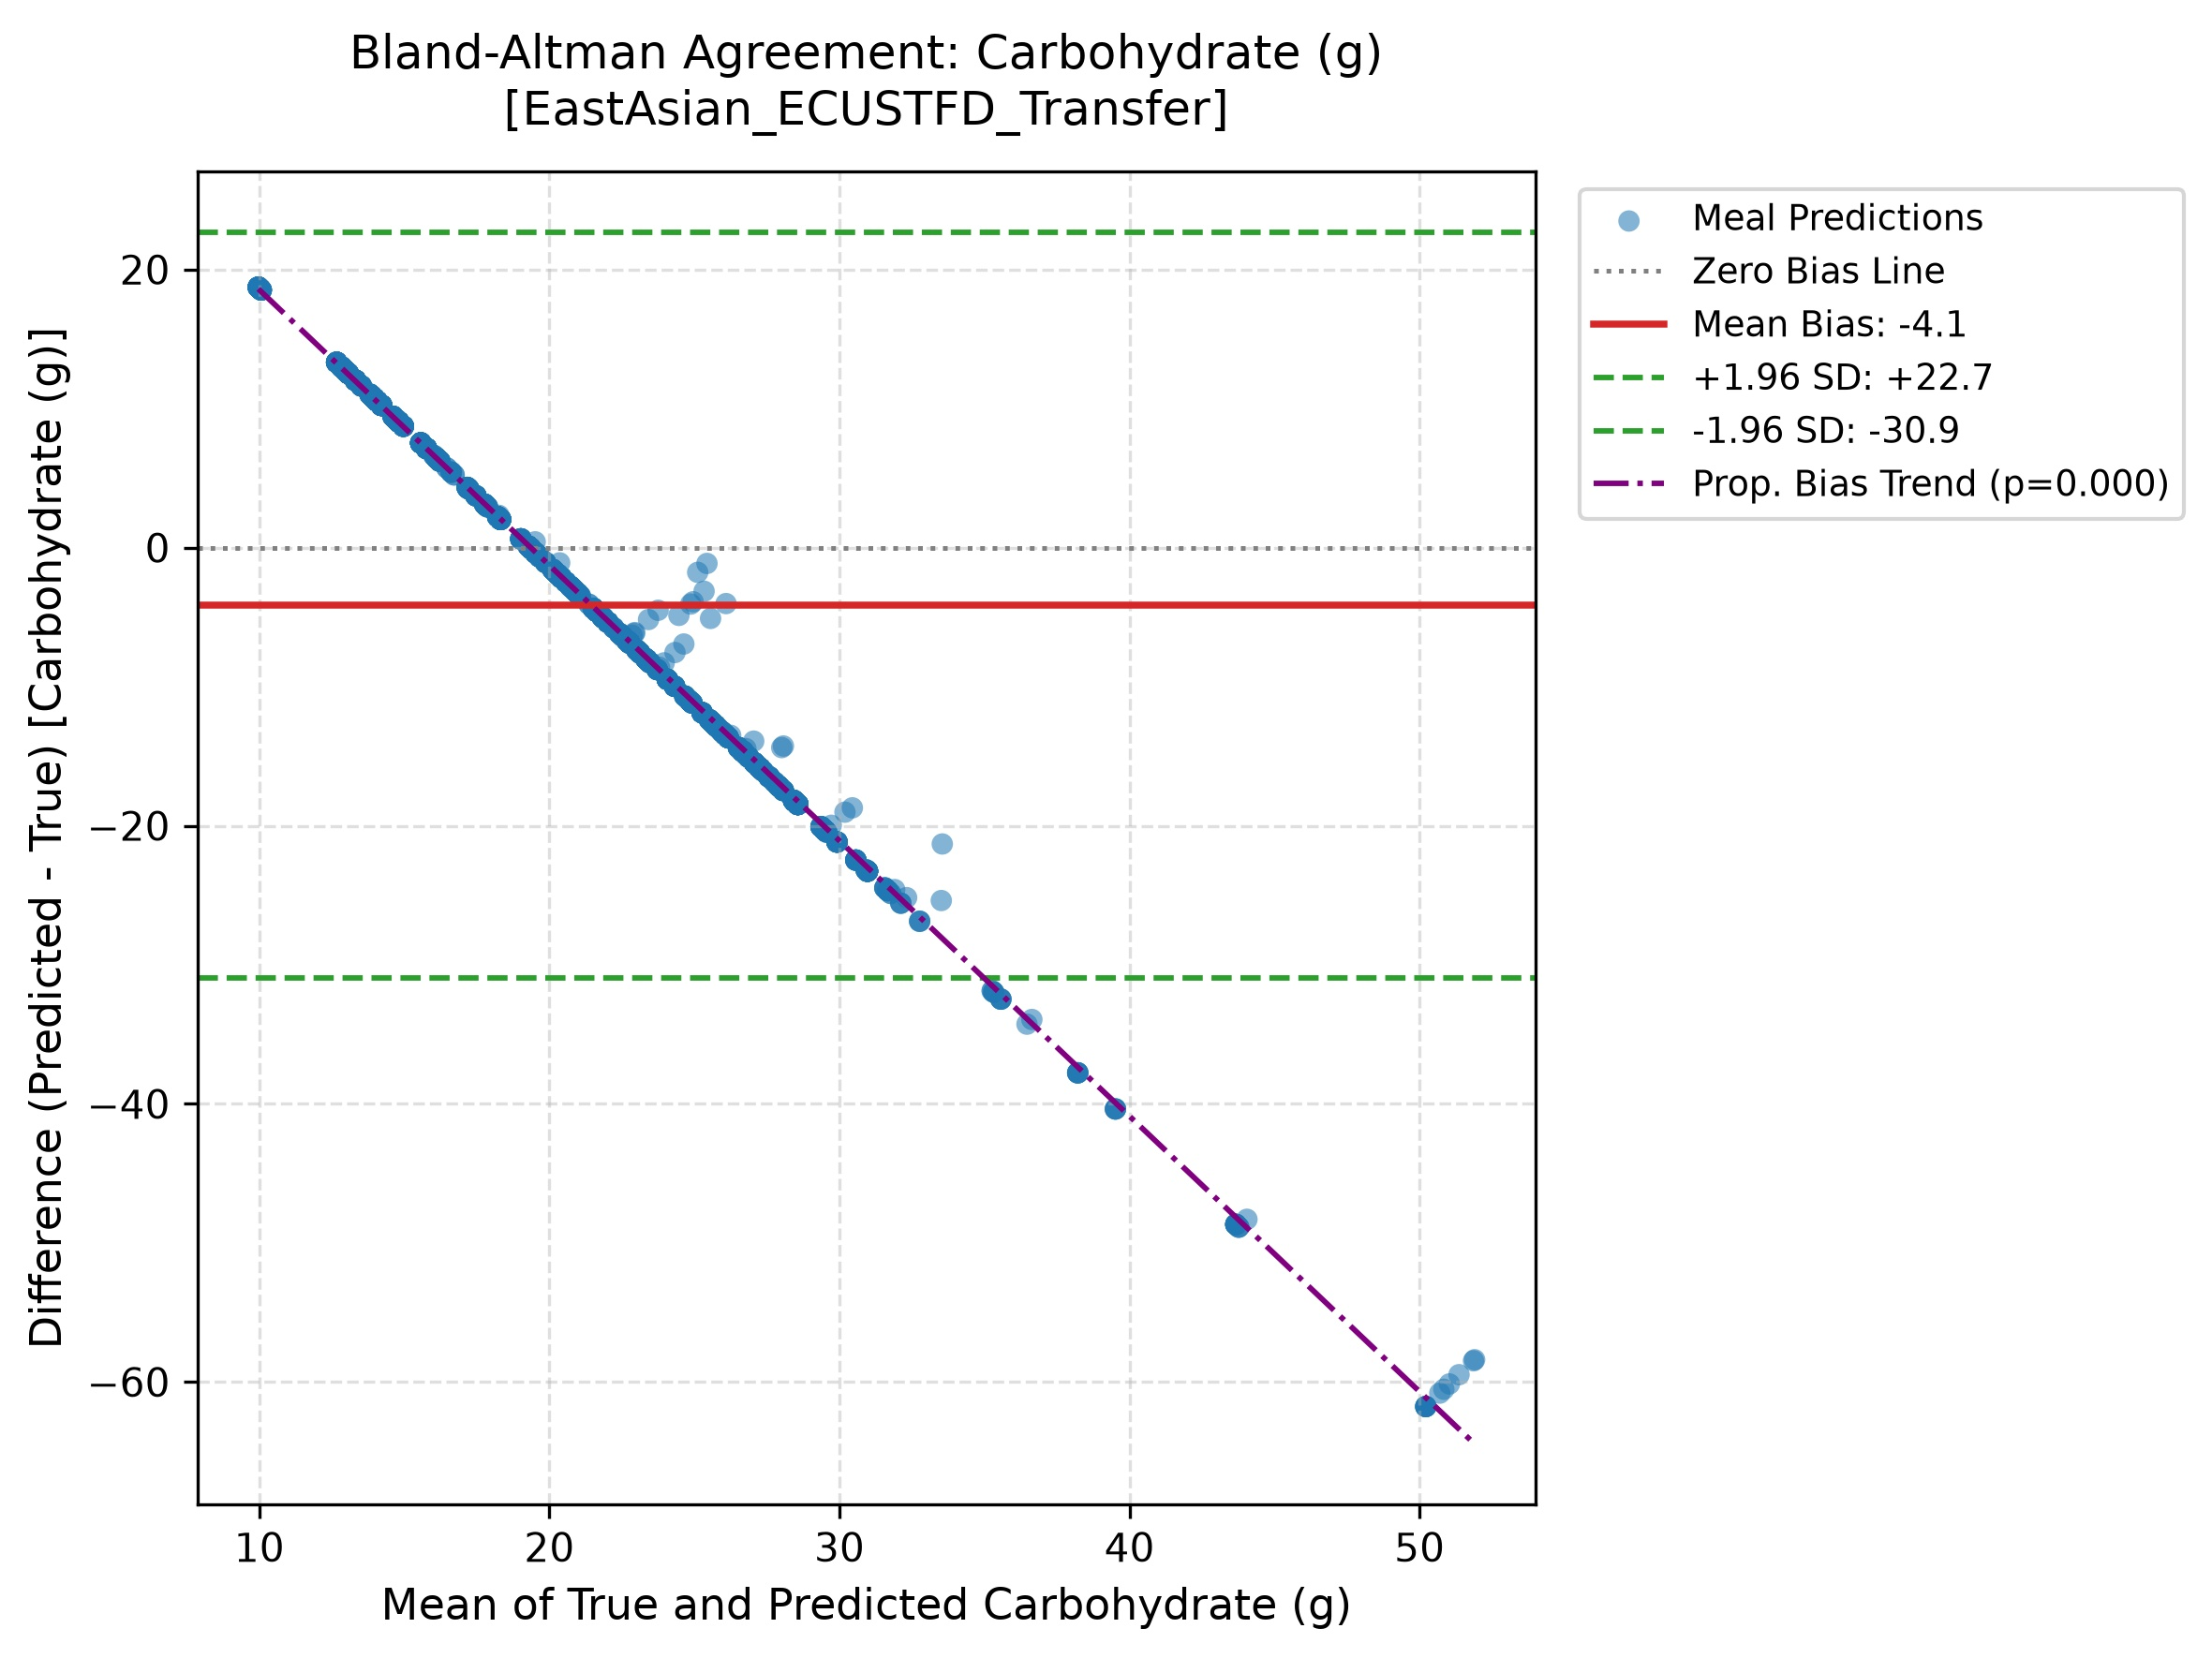
\includegraphics[width=\textwidth]{bland_altman_EastAsian_ECUSTFD_Transfer_carb.jpg}\\
    \small \textbf{(C)} East Asian Transfer
\end{minipage}
\caption{\textbf{Bland-Altman Agreement for Dietary Carbohydrate (g) and Clinical Discrepancy.} Measurement differences ($\hat{y} - y$) plotted against mean values. Note the severe negative mean bias ($-18.2$\,g) and downward proportional trend on South Asian curries and staples, directly endangering diabetic postprandial insulin dosing.}
\label{fig:bland_altman_carb}
\end{figure}

\subsection{Disproportionate Carbohydrate Bias Across Culinary Archetypes}

Stratification of the $1,833$ FoodBD meals into distinct culinary archetypes established whether carbohydrate underestimation in South Asian diets was driven by specific culinary preparation styles or reflected an invariant systemic pathology. Meals were grouped into six culinary categories encompassing ruti flatbread preparations, rice combined with meat or fish curries, traditional savory fried snacks such as beguni, peyaju, singara, and alu-chop, rice accompanied by vegetable or lentil dishes, vegetable and daal gravies, and heterogeneous mixed meal preparations, as summarized in Table~\ref{tab:subgroup_archetypes}.

Across all six culinary categories, the Western-trained vision model exhibited an invariant prediction profile, generating an average predicted carbohydrate output restricted to a narrow interval between $19.8 \pm 1.3$\,g and $22.4 \pm 4.0$\,g regardless of actual dish carbohydrate content. Because network outputs remained anchored to this training prior, the magnitude of directional negative bias was directly proportional to the dish true carbohydrate density.

Traditional Savory Snacks ($N=296$) exhibited the most catastrophic clinical failure. True carbohydrate content averaged $70.1 \pm 31.1$\,g, whereas the network predicted an average of only $22.4 \pm 4.0$\,g, producing a severe negative bias of $-47.68$\,g and an MAE of $48.37$\,g. Clinical safety collapsed to $14.9\%$ within the ADA $\pm 15$\,g window and $17.9\%$ within the $\pm 20$\,g margin, placing over $80\%$ of savory snack consumption in the severe under-bolusing zone. Similarly, Rice combined with Meat/Fish Curries ($N=550$) contained an average of $37.9 \pm 11.5$\,g true carbohydrate compared to a predicted mean of $19.8 \pm 1.5$\,g, inducing a negative bias of $-18.02$\,g with an MAE of $18.72$\,g. Only $34.4\%$ of meals met the ADA $\pm 15$\,g safety tolerance, placing nearly two-thirds of core dinner meals outside safe insulin titration bounds.

In contrast, dishes with lower true carbohydrate density demonstrated higher absolute compliance while retaining persistent underestimation. Ruti / Flatbread Meals ($N=562$) had a true carbohydrate content of $32.1 \pm 12.4$\,g, with predictions averaging $20.4 \pm 2.6$\,g (Mean Bias $-11.71$\,g, MAE $12.93$\,g). Owing to lower portion variance in flatbreads, ADA $\pm 15$\,g compliance reached $68.9\%$, and $\pm 20$\,g compliance reached $84.5\%$. Rice accompanied by Vegetable or Lentil dishes ($N=198$) had an average true carbohydrate of $29.7 \pm 10.6$\,g versus a predicted $19.8 \pm 1.3$\,g (Mean Bias $-9.86$\,g, MAE $10.86$\,g), achieving $76.8\%$ compliance within $\pm 15$\,g and $85.9\%$ within $\pm 20$\,g. Other Mixed Meals ($N=114$) averaged $28.6 \pm 17.6$\,g true carbohydrate with predictions averaging $21.4 \pm 3.4$\,g (Mean Bias $-7.24$\,g, MAE $13.92$\,g, $66.7\%$ ADA compliant). Finally, Vegetable and Daal Gravies ($N=113$) possessed a true carbohydrate baseline of $21.2 \pm 18.7$\,g that closely matched the model training prior ($21.8 \pm 3.2$\,g), yielding a negligible net signed bias ($+0.56$\,g), though wide variance in preparation density maintained an MAE of $16.29$\,g and restricted ADA compliance to $52.2\%$.

These subgroup findings demonstrate that carbohydrate underestimation is not an artifact of random sensor noise, but rather stems from prior dominance that constricts predictions toward Western portion norms. To determine whether this breakdown is driven by misjudging physical portion mass or by failing to infer internal nutrient density, mathematical error decomposition was conducted.

\begin{table}[tbp]
\centering
\small
\caption{\textbf{Subgroup Audit of Carbohydrate Estimation Across South Asian Culinary Archetypes.} Analysis of 1,833 FoodBD meal images stratified by preparation style and staple composition under zero-shot transfer. Best values per column are highlighted in bold.}
\label{tab:subgroup_archetypes}
\vspace{4pt}
\resizebox{\textwidth}{!}{
\begin{tabular}{lrrrrrrr}
\toprule
\textbf{Culinary Archetype} & \textbf{$N$} & \textbf{True Carb (g)} & \textbf{Pred Carb (g)} & \textbf{Mean Bias (g)} & \textbf{MAE (g)} & \textbf{Within $\pm 15$\,g (\%)} & \textbf{Within $\pm 20$\,g (\%)} \\
 & & & & & & \textbf{[ADA Target]} & \textbf{[Clinical Margin]} \\
\midrule
Ruti / Flatbread Meals         & 562 & $32.1 \pm 12.4$ & $20.4 \pm 2.6$ & -11.71 & 12.93 & 68.9 & 84.5 \\
Rice + Meat/Fish Curries       & 550 & $37.9 \pm 11.5$ & $19.8 \pm 1.5$ & -18.02 & 18.72 & 34.4 & 55.3 \\
Traditional Savory Snacks      & 296 & $70.1 \pm 31.1$ & $22.4 \pm 4.0$ & -47.68 & 48.37 & 14.9 & 17.9 \\
Rice + Vegetable/Lentil        & 198 & $29.7 \pm 10.6$ & $19.8 \pm 1.3$ & -9.86  & \textbf{10.86} & \textbf{76.8} & \textbf{85.9} \\
Other Mixed Meals              & 114 & $28.6 \pm 17.6$ & $21.4 \pm 3.4$ & -7.24  & 13.92 & 66.7 & 78.1 \\
Vegetable \& Daal Gravies      & 113 & $21.2 \pm 18.7$ & $21.8 \pm 3.2$ & \textbf{+0.56}  & 16.29 & 52.2 & 74.3 \\
\bottomrule
\end{tabular}
}
\end{table}

\subsection{Mechanistic Error Decomposition: Portion Mass vs. Nutrient Density Collapse}

Orthogonal error decomposition (Eq.~\ref{eq:error_decomposition}) quantitatively separated cross-cultural estimation failures into portion mass deviation versus nutrient density misattribution (Table~\ref{tab:error_decomposition}).

In the Western in-domain cohort ($N=506$), true carbohydrate density ($0.109$\,g/g) was closely tracked by the network ($\hat{D} = 0.082$\,g/g). Portion mass overestimation contributed $+8.80$\,g to total error ($\Delta_{\text{mass}}$), which was balanced by a moderate density underestimation contribution of $-5.23$\,g ($\Delta_{\text{density}}$) and an interaction term of $-2.62$\,g ($\Delta_{\text{interaction}}$). The counterbalancing effect between mass and density errors yielded a net neutral signed bias of $+0.94$\,g.

Conversely, on South Asian meals ($N=1,833$), authentic dishes exhibited a substantially higher true carbohydrate density ($0.192$\,g/g) attributable to concentrated pulses, lentils, and starch gravies. However, the predicted carbohydrate density collapsed to $0.067$\,g/g, remaining virtually identical to the Western cafeteria baseline. Consequently, internal density misattribution drove a large negative deficit of $-25.70$\,g, compounded by a second-order interaction penalty of $-17.65$\,g. Although total dish mass was overestimated ($+25.18$\,g mass contribution), the combined density deficit of $-43.35$\,g completely overwhelmed the mass overestimation, establishing the net negative bias of $-18.18$\,g. This mathematical attribution demonstrates that more than $75\%$ of cross-cultural error arises from internal chemical density blindness (\emph{visual indeterminacy}) rather than surface boundary segmentation errors.

On East Asian images ($N=1,484$), true carbohydrate density was high ($0.230$\,g/g in steamed buns and sweetened snacks), while predicted density averaged $0.089$\,g/g. Portion mass overestimation contributed $+26.80$\,g, which was offset by a $-11.07$\,g density underestimation and a $-19.85$\,g interaction term, resulting in a net signed error of $-4.11$\,g.

This mathematical decomposition confirms that cross-cultural error cannot be resolved merely by improving edge detection or boundary segmentation models. Instead, models require domain-specific density priors, raising the crucial practical question of whether few-shot localized calibration can rectify this density blindness without massive re-annotation campaigns.

\begin{table}[tbp]
\centering
\small
\caption{\textbf{Mathematical Error Decomposition for Dietary Carbohydrate Estimation.} Attribution of total carbohydrate estimation error into portion mass deviation, nutrient density misattribution, and second-order interaction across cohorts ($N=3,823$ total images). Best values per column are highlighted in bold.}
\label{tab:error_decomposition}
\vspace{4pt}
\resizebox{\textwidth}{!}{
\begin{tabular}{lrrrrrrr}
\toprule
\textbf{Target Cohort} & \textbf{$N$} & \textbf{True Density} & \textbf{Pred Density} & \textbf{Total Error} & \textbf{Mass Contrib.} & \textbf{Density Contrib.} & \textbf{Interaction} \\
 & & \textbf{(g/g)} & \textbf{(g/g)} & \textbf{(g)} & \textbf{(g)} & \textbf{(g)} & \textbf{(g)} \\
\midrule
\textbf{Western} (Nutrition5k, In-Domain) & 506 & 0.109 & 0.082 & \textbf{+0.94}  & \textbf{+8.80}  & \textbf{-5.23}  & \textbf{-2.62} \\
\textbf{South Asian} (FoodBD, Transfer)   & 1,833 & 0.192 & 0.067 & -18.18 & +25.18 & -25.70 & -17.65 \\
\textbf{East Asian} (ECUSTFD, Transfer)   & 1,484 & 0.230 & 0.089 & -4.11  & +26.80 & -11.07 & -19.85 \\
\bottomrule
\end{tabular}
}
\end{table}

\subsection{Algorithmic Inequity Mitigation via Few-Shot Calibrated Transfer}

Empirical evaluation of the localized affine recalibration protocol (Eq.~\ref{eq:few_shot_calibration}) on the held-out FoodBD test partition ($N=180$ images with complete visual and nutritional ground truth) established whether systematic cultural bias can be remediated using constrained target-domain sample budgets ($K \in \{20, 50, 100\}$, Table~\ref{tab:few_shot_calibration}).

Under zero-shot evaluation on this independent test partition ($K=0$), the model replicated its severe negative carbohydrate bias ($-18.42$\,g) and poor ADA $\pm 15$\,g safety compliance ($48.3\%$). Energy MAE stood at $151.5$\,kcal.

With a modest localized calibration bank of only $K=20$ annotated meals, energy MAE immediately contracted by $39.2\%$ to $92.1$\,kcal, while carbohydrate bias overcompensated to $+10.53$\,g. Expanding the calibration bank to $K=50$ annotated meals achieved optimal balance: carbohydrate bias contracted from $-18.42$\,g to $-2.81$\,g (an $84.7\%$ reduction in directional bias magnitude), carbohydrate MAE improved from $21.17$\,g to $15.97$\,g (a $24.6\%$ improvement), and ADA $\pm 15$\,g compliance rebounded from $48.3\%$ to $63.9\%$. This $63.9\%$ compliance rate fully matched the $63.8\%$ in-domain Western level. Total energy MAE simultaneously improved by $39.6\%$ (from $151.5$ to $91.5$\,kcal), while compliance within the $\pm 20$\,g clinical margin reached $77.8\%$.

Expanding the calibration set to $K=100$ meals virtually eliminated directional systematic bias ($+0.94$\,g) and established $73.3\%$ safety under the $\pm 20$\,g clinical bolus threshold, with energy MAE remaining stable at $92.8$\,kcal. These findings confirm that while zero-shot cross-cultural deployment of Western-centric models is clinically hazardous, localized calibration using accessible sample sizes ($K=50$ to $100$) provides a viable regulatory pathway to eliminate algorithmic disparities and restore clinical equity.

\begin{table}[tbp]
\centering
\small
\caption{\textbf{Empirical Remediation of Cultural Bias via Few-Shot Localized Calibration.} Clinical carbohydrate safety metrics and energy errors on the independent FoodBD test cohort ($N=180$) across sample budgets ($K=0, 20, 50, 100$). Best values per column are highlighted in bold.}
\label{tab:few_shot_calibration}
\vspace{4pt}
\resizebox{\textwidth}{!}{
\begin{tabular}{lrrrrrr}
\toprule
\textbf{Adaptation Protocol} & \textbf{$K$ Meals} & \textbf{Carb Bias (g)} & \textbf{Carb MAE (g)} & \textbf{ADA Safe $\pm 15$\,g (\%)} & \textbf{Safe $\pm 20$\,g (\%)} & \textbf{Energy MAE (kcal)} \\
\midrule
Zero-Shot Baseline (Western Prior)  & 0   & -18.42 & 21.17 & 48.3 & 61.7 & 151.5 \\
Localized Calibration ($K=20$)       & 20  & +10.53 & 24.11 & 52.2 & 63.3 & 92.1 \\
Localized Calibration ($K=50$)       & 50  & \textbf{-2.81}  & \textbf{15.97} & \textbf{63.9} & \textbf{77.8} & \textbf{91.5} \\
Localized Calibration ($K=100$)      & 100 & \textbf{+0.94}  & 16.63 & 57.8 & 73.3 & 92.8 \\
\bottomrule
\end{tabular}
}
\end{table}

\section{Discussion}

\subsection{Cross-Cultural Vulnerability and Directional Estimation Bias}

Empirical evaluation across diverse cultural dietary cohorts demonstrates that deep learning vision systems for nutritional assessment are not culturally neutral. Transferring multi-task neural architectures trained on Western cafeteria dishes to South Asian and East Asian diets produces systematic, directional estimation bias across multiple nutritional endpoints. Global summary statistics, including mean absolute error and correlation coefficients, obscure these directional distortions. On South Asian meals, the model exhibited a pronounced negative carbohydrate bias of $-18.18$\,g ($p = 8.64 \times 10^{-206}$), accompanied by a collapse in Lin concordance correlation from $0.225$ in-domain to $0.018$ under transfer. Conversely, evaluating the same architecture on East Asian single-item foods produced an energy overestimation bias of $+134.73$\,kcal ($p < 10^{-300}$). These contrasting degradation patterns reveal that deep dietary estimation models do not infer universal physical relationships of food volume and density. Instead, neural networks encode joint statistical distributions that couple visual surface textures with the demographic portion baselines of their initial training environments.

\subsection{Mechanisms of Cultural Bias: Visual Indeterminacy and Prior Dominance}

The asymmetric breakdown observed across food traditions is driven by two interrelated phenomena: visual indeterminacy and Bayesian prior dominance. In standard Western cafeteria meals, food components are predominantly presented as discrete, unblended items arranged on a planar plate, such as sliced grilled meat, steamed vegetables, and whole potato wedges. For such culinary preparations, two-dimensional surface boundaries and visible texture gradients correlate strongly with physical volume, component mass, and macronutrient density. In contrast, South Asian food preparation relies heavily on composite curries, stews, and gravies, in which energy-dense carbohydrates from lentils, pureed pulses, and mashed root vegetables, as well as hidden fats from ghee and mustard oil, are suspended within optically opaque sauces. Because optical cameras record only two-dimensional surface reflectance, the internal chemical concentration of an opaque gravy cannot be resolved from RGB imagery alone. Under this condition of visual indeterminacy, the network defaults to its learned Western training prior ($19.7 \pm 17.5$\,g carbohydrate), generating an invariant prediction profile that fails to reflect actual carbohydrate content. Orthogonal error decomposition confirms this attribution: over $75\%$ of cross-cultural estimation error stems from internal nutrient density collapse rather than geometric portion mass miscalculation.

\subsection{Clinical Safety Hazards in Diabetic Glycemic Management}

The observed directional carbohydrate underestimation introduces immediate clinical hazards for individuals living with diabetes who rely on accurate carbohydrate counting for prandial insulin calculation. In intensive insulin therapy, mealtime rapid-acting insulin boluses are titrated using individualized insulin-to-carbohydrate ratios, conventionally established at one unit of insulin per $10$ to $15$\,g of ingested carbohydrate. A systematic underestimation of $18.2$\,g carbohydrate per meal corresponds to an automatic under-dosing deficit of $1.2$ to $1.8$ units of rapid-acting insulin at every eating occasion. In continuous glucose monitoring profiles, this recurrent shortfall induces acute postprandial glycemic excursions frequently surpassing $180\text{--}250$\,mg/dL ($10.0\text{--}13.9$\,mmol/L), directly eroding time-in-range ($70\text{--}180$\,mg/dL) and accelerating microvascular and macrovascular complications. Under the clinical safety margin established by the American Diabetes Association ($\pm 15$\,g of true carbohydrate), target compliance in South Asian meals dropped from $63.83\%$ in-domain to $49.48\%$. Consequently, more than half of all South Asian meals would receive clinically unsafe bolus recommendations from an uncalibrated vision application. Furthermore, Bland-Altman agreement analysis revealed an expansive downward fan-out, demonstrating that insulin under-dosing risks escalate disproportionately on meals with the highest carbohydrate loads, where discrepancies reach $-40$\,g to $-60$\,g.

Conversely, the positive caloric divergence ($+134.7$\,kcal) observed on East Asian dishes demonstrates an inverted clinical hazard. For patients administering mealtime insulin, overestimating carbohydrate or energy contents prompts excessive prandial insulin delivery, precipitating acute, life-threatening hypoglycemia (plasma glucose $<70$\,mg/dL or $<3.9$\,mmol/L), an acute emergency associated with cognitive dysfunction, adrenergic collapse, seizures, and cardiac arrhythmias. For non-insulin-dependent individuals following medical nutrition therapy, chronic caloric overestimation induces unnecessary dietary restriction, patient anxiety, and potential micronutrient deficits. Therefore, evaluating bidirectional estimation drift is as vital to patient safety as calculating aggregate error magnitudes.

\subsection{The Label Provenance Hierarchy in Nutritional Benchmarking}

A critical methodological insight emerging from this cross-cultural audit is that ground-truth nutrition labels do not represent a homogeneous reference standard. In nutritional epidemiology and digital health, label provenance occupies a distinct methodological hierarchy spanning precision laboratory measurements and field-collected clinical estimations. Laboratory and cafeteria datasets, exemplified by Nutrition5k and ECUSTFD, establish precision physical weighed records by measuring food mass before and after preparation using calibrated digital balances and linking items to laboratory food tables. This paradigm ensures high internal measurement validity, but reflects artificial, highly structured food arrangements unrepresentative of authentic domestic meal preparation.

In contrast, field-collected benchmarks such as FoodBD capture authentic domestic dining patterns, mixed composite gravies, and realistic tableware through dietitian visual estimation linked to regional food composition tables. However, these benchmarks inherit the observational variance of trained dietitians and the standard recipe assumptions embedded in regional food composition databases. Crucially, sensitivity bounds confirm that human dietitian estimation variance cannot explain the observed directional bias. In nutritional literature, registered dietitian visual portion estimates exhibit an observational coefficient of variation of approximately $10\%\text{--}15\%$, distributed stochastically around ground truth. Across $N=1,833$ independent FoodBD dining instances, random observer error would yield symmetric variance rather than a unidirectional carbohydrate deficit of $-18.18$\,g with an extreme significance level ($p = 8.64 \times 10^{-206}$). Even under conservative bounds positing a $+10$\,g systematic overestimation in dietitian labels, an unexplained negative algorithmic deficit exceeding $-8$\,g remains. This confirms that performance degradation is driven primarily by optical indeterminacy, where deep models fail to resolve starch-thickened gravies and submerged pulses, rather than reference label noise. Future dietary AI research must transition from assuming deterministic ground truth toward adopting probabilistic frameworks that explicitly model dietitian estimation variance and regional recipe heterogeneity.

\subsection{Remediation Boundaries: Few-Shot Calibration and Sensor Constraints}

Although zero-shot cross-cultural deployment yields clinically unacceptable error rates, empirical calibration demonstrates that systematic bias can be remediated without extensive re-annotation campaigns. In the independent FoodBD validation cohort, localized affine recalibration with $K=50$ annotated meals reduced carbohydrate bias by $84.7\%$ (from $-18.42$\,g to $-2.81$\,g), reduced carbohydrate MAE by $24.6\%$ (from $21.17$\,g to $15.97$\,g), and restored ADA $\pm 15$\,g compliance to $63.9\%$, matching the $63.8\%$ in-domain Western baseline while reducing energy MAE by $39.6\%$. Nevertheless, several methodological boundaries define the scope of these findings. First, this investigation evaluated standard monocular RGB imagery, which reflects the smartphone technology accessible to global patient populations, but lacks multi-spectral or physical depth channels that could assist in volumetric surface reconstruction. Second, localized recalibration operates at the population cohort level and does not eliminate dish-level variance arising from differing household cooking styles. Third, external validation was conducted across three defined cultural cohorts, and further empirical work is required to establish generalizability across Latin American, African, and Middle Eastern culinary traditions.

\subsection{Actionable Recommendations for Regulatory Governance and Clinical AI Deployment}

To prevent digital health technologies from exacerbating disparities across diverse populations, the empirical findings highlight the necessity of updating regulatory clearance pathways and technical auditing standards. Regulatory frameworks governing Software as a Medical Device, including evaluation pathways through the United States Food and Drug Administration and European medical device authorities, should mandate empirical validation across multi-ethnic dietary cohorts rather than permitting performance certification based solely on Western convenience benchmarks. Evaluating algorithms on ethnically diverse cohorts must become a non-negotiable prerequisite for safety clearance in metabolic disease indications. In parallel, technical performance audits must move beyond symmetric aggregate distance metrics, such as coefficient of determination and mean absolute error, to mandate the reporting of Mean Signed Bias and the proportion of predictions satisfying American Diabetes Association carbohydrate counting safety thresholds ($\pm 15$\,g and $\pm 20$\,g). Reporting directional error distributions guarantees that population-specific systematic biases are detected and audited prior to clinical deployment.

At the interface of clinical deployment and software engineering, digital nutrition applications should disclose the provenance of training data and implement localized few-shot calibration or brief interactive prompts to resolve visual indeterminacy before issuing prandial insulin advice. Integrating concise user clarifications regarding invisible added cooking fats or starch thickeners provides an accessible mechanism to overcome optical indeterminacy while maintaining high user engagement. Combining localized algorithmic calibration with user-in-the-loop verification offers a practical, scalable blueprint to safeguard clinical decision support across global dietary cultures.

\section{Conclusion}

Multi-task deep learning architectures for image-based dietary energy and macronutrient estimation trained on Western cafeteria datasets exhibit severe, directional systematic bias when deployed across different culinary cultures. In zero-shot transfer to South Asian meals, the vision model underestimated dietary carbohydrate by an average of $-18.18$\,g ($p = 8.64 \times 10^{-206}$), causing compliance with American Diabetes Association clinical safety tolerances ($\pm 15$\,g) to decline from $63.83\%$ in-domain to $49.48\%$. Mathematical error decomposition revealed that over $75\%$ of cross-cultural error originates from internal nutrient density collapse rather than physical portion mass deviation, as two-dimensional optical sensors cannot penetrate opaque composite gravies and instead regress to Western training priors. Localized few-shot recalibration using an accessible sample budget of $K=50$ target meals reduced directional carbohydrate bias by $84.7\%$ (from $-18.42$\,g to $-2.81$\,g), lowered energy MAE by $39.6\%$ (from $151.5$ to $91.5$\,kcal), and restored clinical ADA safety compliance to $63.9\%$. These findings establish an empirical foundation and regulatory blueprint for eliminating algorithmic disparities, confirming that culturally contextualized calibration and directional safety audits are indispensable for safe, equitable global deployment of dietary artificial intelligence in clinical care.

\section*{Author Contributions}
Cuicui Liu: Conceptualization, methodology, software, formal analysis, investigation, writing (original draft), supervision, project administration. Huan Peng: Data curation, validation, software, formal analysis, visualization, writing (review and editing). Weijun Liang: Conceptualization, methodology, formal analysis, resources, supervision, project administration, writing (review and editing). All authors contributed to manuscript revision and approved the submitted version.

\section*{Funding}
The authors declare that no financial support was received for the research, authorship, and/or publication of this article.

\section*{Conflict of Interest Statement}
The authors declare that the research was conducted in the absence of any commercial or financial relationships that could be construed as a potential conflict of interest.

\section*{Ethics Approval and Consent to Participate}
This study represents a secondary computational evaluation and statistical audit conducted exclusively on publicly available, de-identified, and open-access dietary benchmarks (Nutrition5k, FoodBD, and ECUSTFD). All primary datasets were collected and published in prior scientific literature in accordance with the Declaration of Helsinki and their respective institutional ethical clearances under open academic research licenses: Nutrition5k is released by Google Research for non-commercial academic research; FoodBD is published under the Creative Commons Attribution 4.0 International license (CC BY 4.0); and ECUSTFD is openly accessible for scientific investigation. No primary human participants were recruited, no identifiable clinical patient records were accessed, and no biological specimens were collected. In accordance with the national ethical regulations for biomedical research involving humans and institutional research ethics guidelines at Changsha Medical University and The Affiliated Changsha Central Hospital, formal institutional review board approval and individual informed consent were exempt for this secondary computational analysis of openly accessible, anonymized public benchmark data.

\section*{Consent to Publish}
All food photographs evaluated in this manuscript are derived from open research benchmark repositories and contain no identifiable personal images, private health details, or biometric patient information. Individual consent to publish was not required.

\section*{Data Availability Statement}
All primary dietary datasets analyzed in this study are publicly accessible research benchmarks. The Nutrition5k benchmark is available through Google Research at \url{https://github.com/google-research-datasets/Nutrition5k}. The FoodBD dataset is accessible via the Mendeley Data repository at \url{https://data.mendeley.com/datasets/xh3ghf3jbg/2}. The ECUSTFD repository is hosted on GitHub at \url{https://github.com/Liang-yc/ECUSTFD-resized-}. Standardized cross-cultural evaluation records and cohort metadata are available within the study repository.

\section*{Code Availability}
The computational evaluation pipelines, Atwater loss implementations, Bland-Altman analysis scripts, and few-shot localized calibration routines are implemented in Python using PyTorch and standard scientific computing libraries. The complete source code is accessible at \url{https://github.com/Hajimi-Sudo/cross-cultural-diet-ai-bias-audit} and is available from the corresponding authors upon reasonable academic request.

\section*{Acknowledgments}
The authors gratefully acknowledge the research teams behind the Nutrition5k, FoodBD, and ECUSTFD benchmarks for compiling and releasing the open dietary repositories that made this cross-cultural evaluation possible.

\bibliographystyle{Frontiers-Vancouver}
\bibliography{references}

\end{document}
